% GRASP: Copyright 1997,1998,1999  Bruce Allen
% $Id: man_stochastic.tex,v 1.11 1999/07/11 21:22:14 ballen Exp $
\section{GRASP Routines: Stochastic background detection}

\subsection{Data File: {\tt detectors.dat}}
\label{subsec:detectors.dat}
\setcounter{equation}0

This file contains site location and orientation information, a 
convenient name for the detector, and filenames for the detector noise 
power spectrum and whitening filter, for 11 different detector sites.
These site are:
\begin{tabbing}
xxxxx\=\kill
\>(1) Hanford, Washington LIGO site,\\ 
\>(2) Livingston, Louisiana LIGO site,\\
\>(3) VIRGO site,\\
\>(4) GEO-600 site,\\
\>(5) Garching site,\\
\>(6) Glasgow site,\\
\>(7) MIT 5 meter interferometer,\\
\>(8) Caltech 40 meter interferometer,\\
\>(9) TAMA-300 site,\\
\>(10) TAMA-20 site,\\ 
\>(11) ISAS-100 site.
\end{tabbing}
As explained below, information for additional detector sites can
be added to {\tt detectors.dat} as needed. [In fact, there are many
additional sites currently in the file -- look at it to see for yourself.
For example, this file and the referenced parameter files now include the
7 distinct stages of ``enhanced LIGO".  Thus a given site, for example
the Hanford Washington LIGO site, has a number of different entries,
corresponding to different noise power spectra.]

The data contained within this file is formatted as follows:
Any line beginning with a {\tt \#} is regarded as a comment.
All other lines are assumed to begin with an integer (which is the site 
identification number) followed by five floating point numbers and three
character strings, each separated by {\it white} space 
(i.e., one or more spaces, which may include tabs).
The first two floating point numbers specify the location of the central 
station (the central vertex of the two detector arms) on the earth's surface:
The first number is the latitude measured in degrees North of the equator; 
the second number is the longitude measured in degrees West of Greenwich, 
England.
The third floating point number specifies the orientation of the first 
arm of the detector, measured in degrees counter-clockwise from true North.
The fourth floating point number specifies the orientation of the second 
arm of the detector, also measured in degrees counter-clockwise from true 
North.
The fifth floating point number is the arm length, in cm.
The three character strings specify: 
(i) a convenient name (e.g., VIRGO or GEO-600) for the detector site, 
(ii) the name of a data file that contains information about the noise 
power spectrum of the detector, and 
(iii) the name of a data file that contains information about the 
spectrum of the whitening filter of the detector.
(We will say more about the content and format of these two data 
files in Secs.~\ref{subsec:noise_power} and \ref{subsec:whiten}.)
The information currently contained in {\tt detectors.dat} is shown
below:

\lgrindfile{Includes/detectors1.tex}

%\noindent
%Note that each individual character string need not be enclosed in quotes, 
%but it should not include any white space.
%Otherwise, if {\tt Hanford-initial} was written as {\tt Hanford initial}, 
%the function {\tt detector\_site()} (which reads 
%the data file {\tt detectors.dat} as input, as described in 
%Sec.~\ref{subsec:detector_site}), would mistakenly interpret 
%{\tt Hanford} as the name of the detector site, and {\tt initial} as the 
%name of the file containing the detector noise power information.

Site information for new (or hypothetical) detectors can be added to 
{\tt detectors.dat} by simply adhering to the above data format.
For example, as the noise in the LIGO detectors improves, one can 
accommodate these changes in {\tt detectors.dat} by adding additional 
lines that have the same site location and orientation information as 
the ``old'' detectors, but refer to different noise power spectra and 
whitening filter data files.
The only other requirement is that the site identification numbers for 
these ``new and improved'' detectors be different from the old site 
identification numbers, so as to avoid any ambiguity.
Explicitly, one could add the following lines to {\tt detectors.dat} 
to include information about the advanced LIGO detectors:

\lgrindfile{Includes/detectors2.tex}

The file {\tt detectors.dat} currently resides in the
{\tt parameters} subdirectory of {\tt GRASP}.
In order for the stochastic background routines and example
programs that are defined in the following sections to be able to
access the information contained in this file, the user must set
the environment variable {\tt GRASP\_PARAMETERS} to point to this
directory.
For example, a command like:\\
{\tt setenv GRASP\_PARAMETERS /usr/local/GRASP/parameters}\\
should do the trick.
If, however, you want to modify this file (e.g., to add another 
detector or to add another noise curve), then just copy the 
{\tt detectors.dat} file to your own home directory, modify it, 
and set the {\tt GRASP\_PARAMETERS} environment variable to point 
to this directory. 
%
\begin{description}
\item{Comment:}
If you happen to find an error in the {\tt detectors.dat} file, 
{\it please} communicate it to the caretakers of GRASP.
\end{description}

\clearpage

\subsection{Function: {\tt detector\_site()}}
\label{subsec:detector_site}
\setcounter{equation}0

{\tt void detector\_site(char *detectors\_file, int site\_choice, 
float site\_parameters[9], char *site\_name, char *noise\_file, 
char *whiten\_file)}\\
%
This function calculates the components of the position vector of the 
central station, and the components of the two vectors that point
along the directions of the detector arms (from the central station to 
each end station), for a given choice of detector site, using information 
contained in an input data file.  This function can also be used to obtain
the latitude, longitude, arm orientations, and arm length of a detector site.
This function also outputs three character strings that
specify the site name, the name of a data file containing the detector noise 
power information, and the name of a data file containing information about 
the detector whitening filter, respectively.

The arguments of {\tt detector\_site()} are:
\begin{description}
%
\item{\tt detectors\_file:} Input.
A character string that specifies the name of a data file
containing detector site information.
This file is most likely the {\tt detectors.dat} data file described
in Sec.~\ref{subsec:detectors.dat}.
If the file is different from {\tt detectors.dat}, it must have the 
same data format as {\tt detectors.dat}, and it must reside in the 
directory pointed to by the {\tt GRASP\_PARAMETERS} environment variable 
(which you may set as you wish).
If you want to use the {\tt detectors.dat} file distributed with
GRASP, use a command like:\\
{\tt setenv GRASP\_PARAMETERS /usr/local/GRASP/parameters}\\
to point to the directory containing this file.  
If you want to modify this file (e.g., to add another detector or 
to add another noise curve), then just copy the {\tt detectors.dat}
file to your own home directory, modify it, and set the 
{\tt GRASP\_PARAMETERS} environment variable to point to this directory. 
%
\item{\tt site\_choice:} Input. 
An integer value used as an index into the input data file.
The absolute value of {\tt site\_choice} should be chosen to match the site 
identification number for one of the detectors contained in this file.
The integer can be positive or negative depending on whether the user
wants the positions of the end stations (positive), or simply the latitude,
longitude, arm orientation and length (negative).
%
\item{\tt site\_parameters:} Output.  If {\tt site\_choice} was positive,
{\tt site\_parameters[0..8]} is an array of nine floating point variables
that define the position of the 
central station of the detector site and the orientation of its two arms.  
The three-vector {\tt site\_parameters[0..2]} are the $(x,y,z)$ components 
(in cm) of the position vector of the central station, as measured in a 
reference frame with the origin at the center of the earth, the 
$z$-axis exiting the North pole, and the $x$-axis passing out the line 
of $0^\circ$ longitude.  
The three-vector {\tt site\_parameters[3..5]} are the $(x,y,z)$ 
components (in cm) of a vector pointing along the direction of the 
first arm (from the central station to the end station).   
The three-vector {\tt site\_parameters[6..8]} are the $(x,y,z)$ 
components (in cm) of a vector pointing along the direction of the 
second arm (from the central station to the end station).
If {\tt site\_choice} was negative, {\tt site\_parameters[0]} contains the
site latitude (degrees north), {\tt site\_parameters[1]} contains the site
longitude (degrees west), {\tt site\_parameters[2]} contains the orientation
of the first arm (degrees CCW from North), {\tt site\_parameters[3]} contains
the orientation of the second arm (degrees CCW from North), and
{\tt site\_parameters[4]} contains the armlength (in cm).  In this case, the
unused elements {\tt site\_parameters[5..7]} are unchanged.
%
\item{\tt site\_name:} Output.
A character string that specifies 
a convenient name (e.g., VIRGO or GEO-600) for the chosen detector site.
%
\item{\tt noise\_file:} Output.
A character string that specifies
the name of a data file containing information about the noise 
power spectrum of the detector.
(See Sec.~\ref{subsec:noise_power} for more details regarding the
content and format of this data file.)
%
\item{\tt whiten\_file:} Output.
A character string that specifies
the name of a data file containing information about the 
spectrum of the whitening filter of the detector.
(See Sec.~\ref{subsec:whiten} for more details regarding the
content and format of this data file.)
\end{description}

{\tt detector\_site()} reads input data from the file specified by
{\tt detectors\_file}.
This file is searched (linearly from top to bottom) until the absolute value of
{\tt site\_choice} matches the site identification number for one of 
the detectors contained in this file.
The site location and orientation information for the chosen
detector site are then read into variables local to {\tt detector\_site()}.
If {\tt site\_choice} was negative, this information is returned in the
array {\tt site\_parameters[]}; otherwise
the values contained in the array {\tt site\_parameters[]} 
are calculated from these input variables using standard equations 
from spherical analytic geometry.
(A correction {\it is} made, however, for the oblateness of the earth, 
using information contained in Ref.~\cite{wortz}.)
The {\tt site\_name}, {\tt noise\_file}, and {\tt whiten\_file}
character strings are simply copied from input data file.
If {\tt site\_choice} does not match any of the site identification 
numbers, {\tt detector\_site()} prints out 
an error message and aborts execution.
%
\begin{description}
\item{Authors:}
Bruce Allen, ballen@dirac.phys.uwm.edu, and Joseph Romano, romano@csd.uwm.edu
\item{Comments:}
None.
\end{description}
\clearpage

\subsection{Comment: noise power spectra for ``advanced" LIGO \& the Cutler-Flanagan model}
\label{subsec:cutlerflanagan}
\setcounter{equation}0
During the years 1992-96, the upcoming LIGO experiment was planned
in two stages, an ``initial" and an ``advanced" stage.  These words
were taken from an important article in {\it Science} \cite{Science92}
which described the LIGO plans.  (The ``advanced" stage has now been
supplanted by a series of seven enhancements and is now described as
``enhanced" LIGO).

During this period 1992-96, research on data analysis algorithms
made use of detector noise curves taken from the {\it Science}
article. Unfortunately two of the figures in the article (Figs. 7 and
10) which gave the noise curve were inconsistent, and also inconsistent
with the parameters given in the article.  The GRASP {\tt parameters/}
directory contains a noise curve corresponding to Fig. 7, and another
noise curve, generally called the ``Cutler and Flanagan" approximation,
which is an approximation to the curve used in Fig. 10.

Note that the noise level in Fig.\ 7 in the Science article
\cite{Science92} is a factor of 3 in $h_{\rm rms}$ [or a factor of $\sim
10$ in $S_n(f)$] lower than that of Fig.\ 10 in between $\sim 10$ Hz and
$\sim 70$ Hz.  Kip Thorne has informed us that Fig.\ 10 is the correct
figure and Fig.\ 7 is in error, and that the error does not appear in
the corresponding figure V.4 of the 1989 LIGO proposal.  The error can
be seen by inserting the parameter values $m = 1000 \, {\rm kg}$, $f_0
= 1 \, {\rm Hz}$, and $Q_0 = 10^9$ given in \cite{Science92} into the
standard equation for suspension thermal noise due to viscous damping,
as given in, e.g., Eq. (4.3) of Reference \cite{finnandchernoff}.
The resulting noise level is a factor of 3 higher than the noise
level shown in Fig.\ 7, and agrees with the noise level of Fig.\ 10.
Note however that the noise curve of Fig.\ 7 has been adopted and used
by several researchers as the ``advanced ligo noise curve", and that the
GRASP ``advanced" advanced noise curve is that of Fig.\ 7.

The Cutler and Flanagan approximation to the advanced ligo noise curve is
\begin{equation}
\label{e:cutflan}
S_n(f) = {1 \over 5} S_0  \left[{f_0^4 \over f^4} +2 \left(1  + {f^2
\over f_0^2} \right) \right]
\end{equation}
for $f \ge 10$ Hz, and $S_n(f) = \infty$ for $f < 10$ Hz, where $S_0
= 3 \times 10^{-48} \, {\rm Hz}^{-1}$ and $f_0 = 70 \,{\rm Hz}$.
This is Eq. (2.1) of Reference \cite{cutler:1994} with $S_0$ replaced
by $S_0/5$ to correct a typo in the published paper.  The noise curve
(\ref{e:cutflan}) is an approximate analytic fit to the advanced noise
curve shown in Fig.\ 10 (not Fig.\ 7) of the LIGO Science article
\cite{Science92}.  
It is the GRASP noise curve {\tt noise\_cutler\_flanagan.dat}.
The accuracy of the fit is fairly good but not a
perfect fit -- in particular the noise curve (\ref{e:cutflan}) is slightly
larger than the noise curve in \cite{Science92} at high frequencies.
A slightly more accurate fit has been obtained by Scott Hughes and
Kip Thorne (quoted in Reference \cite{OwenSathya}), which uses the same
functional form but the slightly different parameter values $f_0 = 75$ Hz
and $S_0 = 2.3 \times 10^{-48}$ with a lower shutoff frequency of $12$ Hz.
\clearpage


\subsection{Function: {\tt noise\_power()}}
\label{subsec:noise_power}
\setcounter{equation}0

{\tt void noise\_power(char *noise\_file, int n, float delta\_f,
double *power)}\\
%
This function calculates the noise power spectrum $P(f)$ of a detector
at a given set of discrete frequency values, using information contained 
in a data file.

The arguments of {\tt noise\_power()} are:
\begin{description}
%
\item{\tt noise\_file:} Input. 
A character string that specifies
the name of a data file containing information about the noise 
power spectrum $P(f)$ of a detector.
Like the {\tt detectors.dat} file described in 
Sec.~\ref{subsec:detectors.dat}, the noise power data file should
reside in the directory pointed to by the {\tt GRASP\_PARAMETERS} 
environment variable (which you may set as you wish).
If you want to use the noise power spectrum data files distributed 
with GRASP, use a command like:\\
{\tt setenv GRASP\_PARAMETERS /usr/local/GRASP/parameters}\\
to point to the directory containing these files.  
If you want to use your own noise power spectrum data files, then
simply set the {\tt GRASP\_PARAMETERS} environment variable to point 
to the directory containing these files.
Note, however, that if a program needs to access {\it both}
detector site information and noise power spectrum data, then all of 
the files containing this information should reside in the {\it same} 
directory.
(A similar remark applies for the whitening filter data files
described in Sec.~\ref{subsec:whiten}.) 
%
\item{\tt n}: Input.
The number $N$ of discrete frequency values at which the noise power
spectrum $P(f)$ is to be evaluated.
%
\item{\tt delta\_f:} Input.
The spacing $\Delta f$ (in Hz) between two adjacent discrete frequency
values: $\Delta f:=f_{i+1}-f_i$.  
%
\item{\tt power:} Output.
{\tt power[0..n-1]} is an array of double precision variables containing 
the values of the noise power spectrum $P(f)$.
These variables have units of ${\rm strain}^2/{\rm Hz}$ (or seconds).
{\tt power[i]} contains the value of $P(f)$ evaluated at the discrete
frequency $f_i=i\Delta f$, where $i=0,1,\cdots,N-1$.
\end{description}

The input data file specified by {\tt noise\_file} contains information 
about the noise power spectrum $P(f)$ of a detector.
The data contained in this file is formatted as follows:
Any line beginning with a {\tt \#} is regarded as a comment.
All other lines are assumed to consist of two floating point numbers
separated by white space.
The first floating point number is a frequency $f$ (in Hz);
the second floating point number is the square root of the 
{\it one-sided} noise power spectrum $P(f)$, evaluated at $f$.
$P(f)$ is defined by equation (3.18) of 
Ref.~\cite{AllenReview}:
%
\begin{equation}
\langle\tilde n{}^*(f)\tilde n(f')\rangle
=:{1\over 2}\delta(f-f')\ P(f)\ .
\label{e:P(f)}
\end{equation}
%
Here $\langle {\ }\rangle$ denotes ensemble average, and $\tilde n(f)$ 
is the frequency spectrum (i.e., Fourier transform) of the strain $n(t)$ 
produced by the noise intrinsic to the detector.
$P(f)$ is a non-negative real function, having units of
${\rm strain}^2/{\rm Hz}$ (or seconds).
It is defined with a factor of 1/2 to agree with the standard
definition used by instrument builders.
The total noise power is the integral of $P(f)$ over all frequencies
from 0 to $\infty$ (not from $-\infty$ to $\infty$).
Hence the name {\it one-sided}.

Since the frequency values contained in the input data file need not 
agree with the desired frequencies $f_i=i\Delta f$,
{\tt noise\_power()} must determine the desired values of the noise
power spectrum by doing an interpolation/extrapolation on the input data.
{\tt noise\_power()} performs a cubic spline interpolation, using the 
{\it Numerical Recipes in C} routines {\tt spline()} and {\tt splint()}. 
{\tt noise\_power()} assumes that the length of the input 
data is $\le 65536$, and it uses boundary conditions for a natural spline 
(i.e., with zero second derivative on the two boundaries).
{\tt noise\_power()} also squares the output of the {\tt splint()}
routine, since the desired values are $P(f)$---and not their square 
roots (which are contained in the input data file).
%
\begin{description}
\item{Authors:}
Bruce Allen, ballen@dirac.phys.uwm.edu, and Joseph Romano, romano@csd.uwm.edu
\item{Comments:}
In order for the cubic spline interpolation routines to 
yield approximations to $P(f)$ that are not contaminated by spurious DC or 
low frequency (e.g., approximately 1 Hz) components, it is important 
that the input data file specified by {\tt noise\_file} contain noise 
power information down to, and including, zero Hz.
This information can be added in ``by hand,'' for example, if the 
experimental data for the noise power spectrum only goes down to 1 Hz.
In this case, setting the values of $\sqrt{P(f)}$ at 
$0.0, 0.1, 0.2, \cdots, 0.9$ Hz equal to its 1 Hz value seems to be 
sufficient.
(See Sec.~\ref{subsec:whiten} for a similar comment regarding
{\tt whiten()}.)
\end{description}
\clearpage

\subsection{Function: {\tt whiten()}}
\label{subsec:whiten}
\setcounter{equation}0

{\tt void whiten(char *whiten\_file, int n, float delta\_f, 
double *whiten\_out)}\\
%
This function calculates the real and imaginary parts of the spectrum
$\tilde W(f)$ of the whitening filter of a detector at a given set of 
discrete frequency values, using information contained in a data file.

The arguments of {\tt whiten()} are:
\begin{description}
%
\item{\tt whiten\_file:} Input. 
A character string that specifies
the name of a data file containing information about the 
spectrum $\tilde W(f)$ of the whitening filter of a detector.
Like the {\tt detectors.dat} and noise power spectrum data files 
described in 
Secs.~\ref{subsec:detectors.dat} and \ref{subsec:noise_power}, 
the whitening filter data file should
reside in the directory pointed to by the {\tt GRASP\_PARAMETERS} 
environment variable (which you may set as you wish).
If you want to use the whitening filter data files distributed with
GRASP, use a command like:\\
{\tt setenv GRASP\_PARAMETERS /usr/local/GRASP/parameters}\\
to point to the directory containing these files.  
If you want to use your own whitening filter data files, then simply
set the {\tt GRASP\_PARAMETERS} environment variable to point to the 
directory containing these files.
Note, however, that if a program also needs to access either detector 
site information or noise power spectrum data, then all of the files 
containing this information should reside in the {\it same} directory.
%
\item{\tt n}: Input.
The number $N$ of discrete frequency values at which the real and 
imaginary parts of the spectrum $\tilde W(f)$ of the whitening filter
are to be evaluated.
%
\item{\tt delta\_f:} Input.
The spacing $\Delta f$ (in Hz) between two adjacent discrete frequency
values: $\Delta f:=f_{i+1}-f_i$.  
%
\item{\tt whiten\_out:} Output.
{\tt whiten\_out[0..2*n-1]} is an array of double precision variables 
containing the values of the real and imaginary parts of the spectrum 
$\tilde W(f)$ of the whitening filter.
These variables have units ${\rm rHz}/{\rm strain}$ 
(or ${\rm sec}^{-1/2}$), which are inverse to the units of the square 
root of the noise power spectrum $P(f)$.
{\tt whiten\_out[2*i]} and {\tt whiten\_out[2*i+1]} contain, respectively, 
the values of the real and imaginary parts of $\tilde W(f)$
evaluated at the discrete frequency $f_i=i\Delta f$, where 
$i=0,1,\cdots,N-1$.
\end{description}

The input data file specified by {\tt whiten\_file} contains information 
about the spectrum $\tilde W(f)$ of the whitening filter of a detector.
The data contained in this file is formatted as follows:
Any line beginning with a {\tt \#} is regarded as a comment.
All other lines are assumed to consist of three floating point numbers,
each separated by white space.
The first floating point number is a frequency $f$ (in Hz).
The second and third floating point numbers are, respectively, the real 
and imaginary parts of the spectrum $\tilde W(f)$, evaluated at $f$.
These last two numbers have units of ${\rm rHz}/{\rm strain}$ 
(or ${\rm sec}^{-1/2}$).
This is because the whitening filter is, effectively, the inverse of 
the amplitude $\sqrt{P(f)}$ of the noise power spectrum.

Since the frequency values contained in the input data file need not 
agree with the desired frequencies $f_i=i\Delta f$, {\tt whiten()} 
must determine the desired values of the real and imaginary parts of the 
spectrum of the whitening filter by doing an
interpolation/extrapolation on the input data.
Similar to {\tt noise\_power()} (see Sec.~\ref{subsec:noise_power}), 
{\tt whiten()} performs a cubic spline interpolation, 
using the {\tt spline()} and {\tt splint()} routines from
{\it Numerical Recipes in C.}
Like {\tt noise\_power()}, {\tt whiten()} assumes that the length of 
the input data is $\le 65536$, and it uses boundary conditions for a 
natural spline.
Unlike {\tt noise\_power()}, {\tt whiten()} does not 
have to square the output of the {\tt splint()}
routine, since the data contained in the input file and the desired
output data both have the same form (i.e., both involve just the real 
and imaginary parts of $\tilde W(f)$).
%
\begin{description}
\item{Authors:}
Bruce Allen, ballen@dirac.phys.uwm.edu, and Joseph Romano, romano@csd.uwm.edu
\item{Comments:}
In order for the cubic spline interpolation routines to 
yield approximations to $\tilde W(f)$ that are not contaminated by spurious 
DC or low frequency (e.g., approximately 1 Hz) components, it is important 
that the input data file specified by {\tt whiten\_file} contain information 
about the whitening filter down to, and including, zero Hz.
This information can be added in ``by hand,'' for example, if the 
experimental data for the spectrum of the whitening filter only goes down 
to 1 Hz.
In this case, setting the values of $\tilde W(f)$ at 
$0.0, 0.1, 0.2, \cdots, 0.9$ Hz equal to their 1 Hz values seems to be 
sufficient.
(See Sec.~\ref{subsec:noise_power} for a similar comment regarding
{\tt noise\_power()}.)

Also, for the initial and advanced LIGO detector noise models, the
spectra $\tilde W(f)$ of the whitening filters contained in the input
data files were constructed by simply inverting the square roots 
of the corresponding noise power spectra $P(f)$.
The spectra of the whitening filters thus constructed are {\it real}.
Although this method of obtaining information about the spectra of the 
whitening filters is fine for simulation purposes, the data contained 
in the actual whitening filter input data files will be obtained 
{\it independently} from that contained in the noise power spectra data 
files, and the spectra $\tilde W(f)$ will in general be complex.
The function {\tt whiten()} described above---and all other
stochastic background routines---allow for this more general form of 
whitening filter data.
\end{description}
\clearpage

\subsection{Function: {\tt overlap()}}
\label{subsec:overlap}
\setcounter{equation}0

{\tt void overlap(float *site1\_parameters, float *site2\_parameters,
int n, float delta\_f, double *gamma12)}\\
%
This function calculates the values of the overlap reduction function 
$\gamma(f)$, which is the averaged product of the response of a pair
of detectors to an isotropic and unpolarized stochastic background of 
gravitational radiation.

The arguments of {\tt overlap()} are:
\begin{description}
%
\item{\tt site1\_parameters:} Input.  
{\tt site1\_parameters[0..8]} is an array of nine floating point variables
that define the position of the central station of the first detector site 
and the orientation of its two arms.  
The three-vector {\tt site1\_parameters[0..2]} are the $(x,y,z)$ components 
(in cm) of the position vector of the central station of the first site, 
as measured in a reference frame with the origin at the center of the earth, 
the $z$-axis exiting the North pole, and the $x$-axis passing out the line 
of $0^\circ$ longitude.  
The three-vector {\tt site1\_parameters[3..5]} are the $(x,y,z)$ 
components (in cm) of a vector pointing along the direction of the 
first arm of the first detector 
(from the central station to the end station).   
The three-vector {\tt site1\_parameters[6..8]} are the $(x,y,z)$ 
components (in cm) of a vector pointing along the direction of the 
second arm of the first detector
(from the central station to the end station).
%
\item{\tt site2\_parameters:} Input.  
{\tt site2\_parameters[0..8]} is an array of nine floating point variables
that define the position of the central station of the second detector site 
and the orientation of its two arms,
in exactly the same format as the previous argument.
%
\item{\tt n:} Input.
The number $N$ of discrete frequency values at which the overlap 
reduction function $\gamma(f)$ is to be evaluated.
%
\item{\tt delta\_f:} Input.
The spacing $\Delta f$ (in Hz) between two adjacent discrete frequency
values: $\Delta f:=f_{i+1}-f_i$.  
%
\item{\tt gamma12:} Output.
{\tt gamma12[0..n-1]} is an array of double precision variables containing 
the values of the overlap reduction $\gamma(f)$ for the two detector sites.
These variables are dimensionless.
{\tt gamma12[i]} contains the value of $\gamma(f)$ evaluated at the discrete
frequency $f_i=i\Delta f$, where $i=0,1,\cdots,N-1$.
\end{description}

The values of $\gamma(f)$ calculated by {\tt overlap()} are defined by 
equation (3.9) of Ref.~\cite{AllenReview}:
%
\begin{equation}
\label{e:overlap}
\gamma(f) := {5 \over 8 \pi} \int_{S^2} d \hat \Omega \>
e^{2 \pi i f \hat \Omega \cdot \Delta \vec x/c }
\left( F_1^+ F_2^+ + F_1^\times F_2^\times \right)\ .
\end{equation}
%
Here $\hat \Omega$ is a unit-length vector on the two-sphere, $\Delta
\vec x$ is the separation vector between the two detector sites, and
$F_i^{+,\times}$ is the response of detector $i$ to the $+$ or $\times$
polarization.  
For the first detector $(i=1)$ one has
%
\begin{equation}
\label{e:detectresponse}
F_1^{+,\times} = {1 \over 2} \left( \hat X_1^a \hat X_1^b - 
\hat Y_1^a \hat Y_1^b \right)e_{ab}^{+,\times}(\hat \Omega)\ ,
\end{equation}
%
where the directions of the first detector's arms are defined by 
$\hat X_1^a$ and $\hat Y_1^a$, and $e_{ab}^{+,\times}(\hat \Omega)$ are 
the spin-two polarization tensors for the ``plus" and ``cross" 
polarizations, respectively.  
(A similar expression can be written down for the second detector.)
The normalization of $\gamma(f)$ is determined by the following statement:  
For coincident and coaligned detectors (i.e., for two detectors located 
at the same place, with both pairs of arms pointing in the same directions),
$\gamma(f)=1$ for all frequencies.
%
\begin{description}
\item{Authors:}
Bruce Allen, ballen@dirac.phys.uwm.edu, and Joseph Romano, romano@csd.uwm.edu
\item{Comments:}
None.
\end{description}
\clearpage

%\subsection{Function: {\tt normalize()}} 
%\label{subsec:normalize}
%\setcounter{equation}0

%{\tt void normalize(float *v)}\\
%%
%This function normalizes a 3-vector $\vec v:=(v_x,v_y,v_z)$ to unit 
%length with respect to the inner product
%$\vec v\cdot\vec v:=v_x^2+v_y^2+v_z^2$.
%This function is called by {\tt overlap()} when constructing unit 
%vectors in the directions of the detector arms.

%The arguments of {\tt normalize()} are:
%\begin{description}
%%
%\item{\tt v:} Input/Output. 
%{\tt v[0..2]} is an array of three floating point variables containing 
%the $(x,y,z)$ components of the input vector $\vec v$.
%The output of {\tt normalize()} are the components of $\vec v$, 
%after it has been normalized to unit length.
%\end{description}
%%
%\begin{description}
%\item{Authors:}
%Bruce Allen, ballen@dirac.phys.uwm.edu, and Joseph Romano, romano@csd.uwm.edu
%\item{Comments:}
%None.
%\end{description}
%\clearpage

\subsection{Example: {\tt overlap} program}
\label{subsec:example_overlap}
\setcounter{equation}0

The following example program shows one way of combining the functions
{\tt detector\_site()} and {\tt overlap()} to calculate 
the overlap reduction function $\gamma(f)$ for a given pair of detectors.
In particular, we calculate $\gamma(f)$ for the Hanford, WA and Livingston, 
LA LIGO detector sites.
The resulting overlap reduction function data is stored as two columns 
of double precision numbers ($f_i$ and $\gamma(f_i)$) in the file 
{\tt LIGO\_overlap.dat}.
Here $f_i=i\Delta f$ with $i=0,1,\cdots,N-1$.
The values of $N$ and $\Delta f$ are input parameters to the program,
which the user can change if he/she desires.
(See the {\tt \#define} statements listed at the beginning of the program.)
Also, by changing the site location identification numbers and the
output file name, the user can calculate and save
the overlap reduction function for {\it any} pair of detectors---e.g.,  
the Hanford, WA LIGO detector and the GEO-600 detector; the GEO-600 
and VIRGO detector; the Garching and Glasgow detectors; etc.
The overlap reduction function data that is stored in the file can 
then be displayed with {\tt xmgr}, for example.
(See Fig.~\ref{f:f1}.)

\lgrindfile{Includes/overlap.tex}

\begin{figure}[h]
\begin{center}
\epsfig{file=Figures/f1_sb.ps,angle=-90,width=5in}
\caption{\label{f:f1}
The overlap reduction function $\gamma(f)$ for the Hanford, WA and 
Livingston, LA LIGO detector pair.}
\end{center}
\end{figure}

\clearpage

\subsection{Function: {\tt get\_IFO12()}}
\label{subsec:get_IFO12}
\setcounter{equation}0

{\tt get\_IFO12(FILE *fp1, FILE *fp2, FILE *fp1lock, FILE *fp2lock, 
int n, float *out1, float *out2, float *srate1, float *srate2)}\\
%
This function gets real interferometer output (IFO) data from two 
detector sites.

The arguments of {\tt get\_IFO12()} are:
\begin{description}
%
\item{\tt fp1:} Input. 
A pointer to a file that contains the interferometer output (IFO) data 
produced by the first detector.
%
\item{\tt fp2:} Input. 
A pointer to a file that contains the interferometer output (IFO) data 
produced by the second detector.
%
\item{\tt fp1lock:} Input.
A pointer to a file that contains the TTL lock signal for the 
interferometer output produced by the first detector.
%
\item{\tt fp2lock:} Input.
A pointer to a file that contains the TTL lock signal for the 
interferometer output produced by the second detector.
%
\item{\tt n:} Input.
The number $N$ of data points to be retrieved.
%
\item{\tt out1:} Output.
{\tt out1[0..n-1]} is an array of floating point variables containing
the values of the interferometer output produced by the first detector.
These variables have units of ADC counts. 
{\tt out1[i]} contains the value of the whitened data stream $o_1(t)$
evaluted at the discrete time $t_i=i\Delta t_1$, where 
$i=0,1,\cdots,N-1$ and $\Delta t_1$ is the sampling period of the
first detector, defined below.
%
\item{\tt out2:} Output.
{\tt out2[0..n-1]} is an array of floating point variables containing
the values of the interferometer output produced by the second detector,
in exactly the same format as the previous argument.
%
\item{\tt srate1:} Output.
The sample rate $\Delta f_1$ (in Hz) of the first detector.
$\Delta t_1:=1/\Delta f_1$ (in sec) is the corresponding sampling 
period of the first detector.
%
\item{\tt srate2:} Output.
The sample rate $\Delta f_2$ (in Hz) of the second detector.
$\Delta t_2:=1/\Delta f_2$ (in sec) is the corresponding sampling 
period of the second detector.
\end{description}

{\tt get\_IFO12()} consists effectively of two calls to 
{\tt get\_data()}, which is described in detail in 
Sec.~\ref{subsec:get_data}
It prints out a warning message if no data remains for one or
both detectors.
For that case, both {\tt out1[]} and {\tt out2[]} are set to 
zero.
%
\begin{description}
\item{Authors:}
Bruce Allen, ballen@dirac.phys.uwm.edu, and Joseph Romano, romano@csd.uwm.edu
\item{Comments:} 
Currently, {\tt get\_IFO12()} calls {\tt get\_data()}
and {\tt get\_data2()}, where {\tt get\_data2()} is simply a copy of the
{\tt get\_data()} routine.  
{\tt get\_data()} should eventually be modified so that it can handle
simultaneous requests for data from more than one detector.
After this change is made, the function {\tt get\_data2()} should be 
removed.
\end{description}
\clearpage

\subsection{Function: {\tt simulate\_noise()}}
\label{subsec:simulate_noise}
\setcounter{equation}0

{\tt void simulate\_noise(int n, float delta\_t, double *power, 
double *whiten\_out, float *out, int *pseed)}\\
%
This function simulates the generation of noise intrinsic to a detector.
The output is a (not necessarily continuous-in-time)
whitened data stream $o(t)$ representing the detector output when 
only detector noise is present.

The arguments of {\tt simulate\_noise()} are:
\begin{description}
%
\item{\tt n:} Input. 
The number $N$ of data points corresponding to an observation
time $T:=N\ \Delta t$, where 
$\Delta t$ is the sampling period of the detector, defined below.
$N$ should equal an integer power of 2.
%
\item{\tt delta\_t:} Input.  
The sampling period $\Delta t$ (in sec) of the detector. 
%
\item{\tt power:} Input.  
{\tt power[0..n/2-1]} is an array of double precision variables 
containing the values of the noise power spectrum $P(f)$ of the 
detector.
These variables have units of ${\rm strain}^2/{\rm Hz}$ (or seconds).
{\tt power[i]} contains the value of $P(f)$ evaluated at the discrete
frequency $f_i=i/(N\Delta t)$, where $i=0,1,\cdots,N/2-1$.
%
\item{\tt whiten\_out:} Input.
{\tt whiten\_out[0..n-1]} is an array of double precision variables 
containing the values of the real and imaginary parts of the spectrum 
$\tilde W(f)$ of the whitening filter of the detector.
These variables have units ${\rm rHz}/{\rm strain}$ 
(or ${\rm sec}^{-1/2}$), which are inverse to the units of the square 
root of the noise power spectrum $P(f)$.
{\tt whiten\_out[2*i]} and {\tt whiten\_out[2*i+1]} contain, respectively, 
the values of the real and imaginary parts of $\tilde W(f)$
evaluated at the discrete frequency $f_i=i/(N\Delta t)$, where 
$i=0,1,\cdots,N/2-1$.
%
\item{\tt out:} Output.  
{\tt out[0..n-1]} is an array of floating point variables containing
the values of the whitened data stream $o(t)$ representing the 
output of the detector when only detector noise is present.
$o(t)$ is the convolution of detector whitening filter $W(t)$
with the noise $n(t)$ intrinsic to the detector.
The variables {\tt out[]} have units of rHz (or ${\rm sec}^{-1/2}$),
which follows from the definition of $n(t)$ as a strain and
$\tilde W(f)$ as the ``inverse'' of the square root
of the noise power spectrum $P(f)$.
{\tt out[i]} contains the value of $o(t)$ evaluated at the discrete 
time $t_i=i\Delta t$, where $i=0,1,\cdots,N-1$.
%
\item{\tt pseed:} Input.  
A pointer to a seed value, which is used by the random number generator
routine.
\end{description}

{\tt simulate\_noise()} simulates the generation of noise intrinsic 
to a detector in the following series of steps:
%
\begin{itemize}
\item[(i)] It first constructs random variables 
$\tilde n(f_i)$ in the frequency domain that have zero mean 
and satisfy:
%
\begin{equation}
\langle \tilde n^*(f_i)\tilde n(f_j)\rangle=
{1\over 2}\ T\ \delta_{ij}\ P(f_i)\ ,\\
\end{equation}
%
where $\langle\ \rangle$ denotes ensemble average.
The above equation is just the discrete frequency version of 
Eq.~(\ref{e:P(f)}).
This equation can be realized by setting
%
\begin{equation}
\tilde n(f_i)={1\over 2}\sqrt{T}\ P^{1/2}(f_i)\ (u_i+i v_i)\ ,
\end{equation}
%
where $u_i$ and $v_i$ 
are statistically independent (real) Gaussian random variables, 
each having zero mean and unit variance.
These Gaussian random variables are produced by calls to the 
{\it Numerical Recipes in C} random number generator routine
{\tt gasdev()}.
%
\item[(ii)] {\tt simulate\_noise()} then whitens the data
in the frequency domain by multiplying $\tilde n(f_i)$ by the 
frequency components $\tilde W(f_i)$ of the whitening filter
of the detector:
%
\begin{equation}
\tilde o(f_i):=\tilde n(f_i)\ \tilde W(f_i)\ .
\end{equation}
%
This (complex) multiplication in the frequency domain corresponds
to the convolution of $n(t)$ and $W(t)$ in the time domain.
By convention, the DC (i.e., zero frequency) and Nyquist critical
frequency components of $\tilde o(f_i)$ are set to zero.
%
\item[(iii)] The final step consists of Fourier transforming the
frequency components $\tilde o(f_i)$ into the time domain to obtain 
the whitened data stream $o(t_i)$.
Here $t_i=i\Delta t$ with $i=0,1,\cdots,N-1$.
\end{itemize}
%
\begin{description}
\item{Authors:}
Bruce Allen, ballen@dirac.phys.uwm.edu, and Joseph Romano, romano@csd.uwm.edu
\item{Comments:}
In the context of stochastic background simulations, it would be
more efficient to simulate the noise at {\it two} detectors simultaneously.
Since the time-series data are real, the two Fourier transforms that 
would need to be performed in step (iii) could be done simultaneously. 
However, for modularity of design, and to simulate noise for 
``single-detector'' gravity-wave searches, we decided to write the above 
routine instead.
\end{description}
\clearpage

\subsection{Function: {\tt simulate\_sb()}}
\label{subsec:simulate_sb}
\setcounter{equation}0

{\tt void simulate\_sb(int n, float delta\_t, float omega\_0, float f\_low,
float f\_high, double *gamma12, double *whiten1, double *whiten2, 
float *out1, float *out2, int *pseed)}\\
%
This function simulates the generation of an isotropic and unpolarized
stochastic background of gravitational radiation having a constant 
frequency spectrum: 
$\Omega_{\rm gw}(f)=\Omega_0$ for $f_{\rm low}\le f \le f_{\rm high}$.
The outputs are (not necessarily continuous-in-time)
whitened data stream $o_1(t)$ and $o_2(t)$ representing the detector 
outputs when only a stochastic background signal is present.

The arguments of {\tt simulate\_sb()} are:
\begin{description}
%
\item{\tt n:} Input. 
The number $N$ of data points corresponding to an observation
time $T:=N\ \Delta t$, where
$\Delta t$ is the sampling period of the detectors, defined below.
$N$ should equal an integer power of 2.
%
\item{\tt delta\_t:} Input.  
The sampling period $\Delta t$ (in sec) of the detectors. 
%
\item{\tt omega\_0:} Input.  
The constant value $\Omega_0$ (dimensionless) of the frequency 
spectrum $\Omega_{\rm gw}(f)$ for the stochastic background:
%
\[
\Omega_{\rm gw}(f)=\left\{
\begin{array}{cl}
\Omega_0 & \quad f_{\rm low}\le f \le f_{\rm high}\\
0        & \quad {\rm otherwise.}
\end{array}
\right.
\]
%
$\Omega_0$ should be greater than or equal to zero.
%
\item{\tt f\_low:} Input.  
The frequency $f_{\rm low}$ (in Hz) below which the spectrum 
$\Omega_{\rm gw}(f)$ of the stochastic background is zero.
$f_{\rm low}$ should lie in the range $0\le f_{\rm low}\le f_{\rm Nyquist}$, 
where $f_{\rm Nyquist}$ is the Nyquist critical frequency. 
(The Nyquist critical frequency is defined by 
$f_{\rm Nyquist}:=1/(2\Delta t)$, 
where $\Delta t$ is the sampling period of the detectors.)
$f_{\rm low}$ should also be less than or equal to $f_{\rm high}$.
%
\item{\tt f\_high:} Input.  
The frequency $f_{\rm high}$ (in Hz) above which the spectrum 
$\Omega_{\rm gw}(f)$ of the stochastic background is zero.
$f_{\rm high}$ should lie in the range $0\le f_{\rm high}\le f_{\rm Nyquist}$.
It should also be greater than or equal to $f_{\rm low}$.
%
\item{\tt gamma12:} Input.
{\tt gamma12[0..n/2-1]} is an array of double precision variables 
containing the values of the overlap reduction function $\gamma(f)$ 
for the two detector sites.
These variables are dimensionless.
{\tt gamma12[i]} contains the value of $\gamma(f)$ evaluated at the 
discrete frequency $f_i=i/(N\Delta t)$, where $i=0,1,\cdots,N/2-1$.
%
\item{\tt whiten1:} Input.
{\tt whiten1[0..n-1]} is an array of double precision variables 
containing the values of the real and imaginary parts of the spectrum 
$\tilde W_1(f)$ of the whitening filter of the first detector.
These variables have units ${\rm rHz}/{\rm strain}$ 
(or ${\rm sec}^{-1/2}$), which are inverse to the units of the square 
root of the noise power spectrum $P_1(f)$.
{\tt whiten1[2*i]} and {\tt whiten1[2*i+1]} contain, respectively, 
the values of the real and imaginary parts of $\tilde W_1(f)$
evaluated at the discrete frequency $f_i=i/(N\Delta t)$, where 
$i=0,1,\cdots,N/2-1$.
%
\item{\tt whiten2:} Input. 
{\tt whiten2[0..n-1]} is an array of double precision variables 
containing the values of the real and imaginary parts of the spectrum 
$\tilde W_2(f)$ of the whitening filter of the second detector,
in exactly the same format as the previous argument.
%
\item{\tt out1:} Output.  
{\tt out1[0..n-1]} is an array of floating point variables containing
the values of the whitened data stream $o_1(t)$ representing the 
output of the first detector when only a stochastic background signal 
is present.
$o_1(t)$ is the convolution of detector whitening filter $W_1(t)$
with the gravitational strain $h_1(t)$.
The variables {\tt out1[]} have units of rHz (or ${\rm sec}^{-1/2}$),
which follows from the definition of $h_1(t)$ as a strain and
$\tilde W_1(f)$ as the ``inverse'' of the square root 
of the noise power spectrum $P_1(f)$.
{\tt out1[i]} contains the value of $o_1(t)$ evaluated at the discrete 
time $t_i=i\Delta t$, where $i=0,1,\cdots,N-1$.
%
\item{\tt out2:} Output.  
{\tt out2[0..n-1]} is an array of floating point variables containing
the values of the whitened data stream $o_2(t)$ representing the 
output of the second detector when only a stochastic background signal 
is present,
in exactly the same format as the previous argument.
%
\item{\tt pseed:} Input.  
A pointer to a seed value, which is used by the random number generator
routine.
\end{description}

{\tt simulate\_sb()} simulates the generation of an isotropic and
unpolarized stochastic background of gravitational radiation having
a constant frequency spectrum 
$\Omega_{\rm gw}(f)=\Omega_0$ for $f_{\rm low}\le f\le f_{\rm high}$
in the following series of steps:
%
\begin{itemize}
\item[(i)] It first constructs random variables
$\tilde h_1(f_i)$ and $\tilde h_2(f_i)$
in the frequency domain that have zero mean and satisfy:
%
\begin{eqnarray}
\langle \tilde h_1^*(f_i)\tilde h_1(f_j)\rangle&=&
{1\over 2}\ T\ \delta_{ij}\ {3H_0^2\over 10\pi^2}\ f_i^{-3}\ \Omega_0
\label{eq:e1}\\
\langle \tilde h_2^*(f_i)\tilde h_2(f_j)\rangle&=&
{1\over 2}\ T\ \delta_{ij}\ {3H_0^2\over 10\pi^2}\ f_i^{-3}\ \Omega_0
\label{eq:e2}\\
\langle \tilde h_1^*(f_i)\tilde h_2(f_j)\rangle&=&
{1\over 2}\ T\ \delta_{ij}\ {3H_0^2\over 10\pi^2}\ f_i^{-3}\ \Omega_0
\ \gamma(f_i)\ ,
\end{eqnarray}
%
where $\langle\ \rangle$ denotes ensemble average.
Here $\tilde h_1(f_i)$ and $\tilde h_2(f_i)$ 
are the Fourier components of the gravitational strains
$h_1(t)$ and $h_2(t)$ at the two detectors.
The above equations are the discrete frequency versions of equation
(3.17) of Ref.~\cite{AllenReview}, with $\Omega_{\rm gw}(f)=\Omega_0$ for
$f_{\rm low}\le f\le f_{\rm high}$.
They can be realized by setting
%
\begin{eqnarray}
\tilde h_1(f_i)&=&{1\over 2}\sqrt{T}\ \left({3H_0^2\over 10\pi^2}\right)^{1/2}
f_i^{-3/2}\ \Omega_0^{1/2}\  (x_{1i} + i y_{1i})\\
\tilde h_2(f_i)&=&\tilde h_1(f_i)\ \gamma(f_i)+\\
&&{1\over 2}\sqrt{T}\ \left({3H_0^2\over 10\pi^2}\right)^{1/2}
f_i^{-3/2}\ \ \Omega_0^{1/2}\ 
\sqrt{1-\gamma^2(f_i)}\ (x_{2i}+i y_{2i})\ ,
\label{eq:eel}
\end{eqnarray}
%
where 
$x_{1i}$, $y_{1i}$, $x_{2i}$, and $y_{2i}$ are statistically 
independent (real) Gaussian random variables, each having zero mean 
and unit variance.
(Note: The $x_{1i}$, $y_{1i}$, $x_{2i}$, and $y_{2i}$ random
variables are statistically independent of the $u_i$ and $v_i$ 
random variables defined in Sec.~\ref{subsec:simulate_noise}.) 
These Gaussian random variables are produced by calls to 
the {\it Numerical Recipes in C} random number generator routine 
{\tt gasdev()}.
Note also that the second term of $\tilde h_2(f_i)$ (which is
proportional to $\sqrt{1-\gamma^2(f_i)}$) is needed to obtain equation
(\ref{eq:e2}).
Without this term, $\langle\tilde h_2^*(f_i)\tilde h_2(f_j)\rangle$ would
include an additional (unwanted) factor of $\gamma^2(f_i)$.
%
\item[(iii)] {\tt simulate\_sb()} then whitens the data
in the frequency domain by multiplying
$\tilde h_1(f_i)$ and $\tilde h_2(f_i)$ by the frequency components
$\tilde W_1(f_i)$ and $\tilde W_2(f_i)$ of the whitening filters
of the two detectors:
%
\begin{eqnarray}
\tilde o_1(f_i)&:=&\tilde h_1(f_i)\ \tilde W_1(f_i)\\
\tilde o_2(f_i)&:=&\tilde h_2(f_i)\ \tilde W_2(f_i)\ .
\end{eqnarray}
%
This (complex) multiplication in the frequency domain corresponds
to the convolution of $h_1(t)$ and $W_1(t)$, and $h_2(t)$ and $W_2(t)$
in the time domain.
By convention, the DC (i.e., zero frequency) and Nyquist critical
frequency components of $\tilde o_1(f_i)$ and $\tilde o_2(f_i)$
are set to zero.
%
\item[(iii)] The final step consists of Fourier transforming the
frequency components $\tilde o_1(f_i)$ and $\tilde o_2(f_i)$ into the 
time domain to obtain the whitened data streams
$o_1(t_i)$ and $o_2(t_i)$.
Here $t_i=i\Delta t$ with $i=0,1,\cdots,N-1$.
Since $\tilde o_1^*(f_i)$ and $\tilde o_2^*(f_i)$ are the Fourier
transforms of real data sets, the two Fourier transforms can be 
performed simultaneously.
\end{itemize}
%
\begin{description}
\item{Authors:}
Bruce Allen, ballen@dirac.phys.uwm.edu, and Joseph Romano, romano@csd.uwm.edu
\item{Comments:}
Although it is possible and more efficient to write a single function to 
simulate the generation of a stochastic background and intrinsic detector 
noise simultaneously, we have chosen---for the sake of modularity---to 
write separate functions to perform these two tasks separately.
(See also the comment at the end of Sec.~\ref{subsec:simulate_noise}.)
\end{description}
\clearpage

\subsection{Function: {\tt combine\_data()}}
\label{subsec:combine_data}
\setcounter{equation}0

{\tt void combine\_data(int which, int n, float *in1, float *in2, 
float *out)}\\
%
This low-level function takes two arrays as input, shifts them by half 
their length, and combines them with one another and with data stored in 
an internally-defined static buffer to produce output data that is 
continuous from one call of {\tt combine\_data()} to the next.

The arguments of {\tt combine\_data()} are:
\begin{description}
%
\item{\tt which:} Input.
An integer variable specifying which internally-defined static
buffer should be used when combining the input arrays with data
saved from a previous call.
The allowed values are $1\le{\tt which}\le 16$.
\item{\tt n:} Input. 
The number $N$ of data points contained in the input and output arrays.
$N$ is assumed to be even.
%
\item{\tt in1:} Input.  
{\tt in1[0..n-1]} is an array of floating point variables containing
the values of the first input array.
%
\item{\tt in2:} Input.  
{\tt in2[0..n-1]} is an array of floating point variables containing
the values of the second input array.
%
\item{\tt out:} Output.  
{\tt out[0..n-1]} is an array of floating point variables 
containing the output data, which is continuous from one call of
{\tt combine\_data()} to the next.
%
\end{description}

{\tt combine\_data()} produces continuous output data by modifying 
the appropriately chosen static buffer {\tt buf[0..3*n/2-1]} as follows:
%
\begin{eqnarray}
&&{\tt buf[i]+=sin[i*M\_PI/n]*in1[i]}\quad{\rm for}\quad
{\tt 0}\le{\tt i}\le{\tt n/2-1}\nonumber\\ 
&&{\tt buf[i]+=sin[i*M\_PI/n]*in1[i]+sin[(i-n/2)*M\_PI/n]*in2[i-n/2]}
\quad{\rm for}\quad{\tt n/2}\le{\tt i}\le{\tt n-1}\nonumber\\ 
&&{\tt buf[i]+=sin[(i-n/2)*M\_PI/n]*in2[i-n/2]}\quad{\rm for}\quad
{\tt n}\le{\tt i}\le{\tt 3*n/2-1}\ .\nonumber
\end{eqnarray} 
%
The values of the output array {\tt out[0..n-1]} are taken from the 
first two-thirds of the buffer, while the last one-third of the buffer
is copied to the first third of the buffer in preparation for the 
next call.
When this is complete, the last two-thirds of the buffer is cleared.

One nice feature of combining the data with a sine function 
(rather than with a triangle function, for example) is that if the
input data represent statistically independent, stationary random 
processes having zero mean and the same variance, then the output 
data will also have zero mean and the same variance.
This is a consequence of the trigonometric identity
%
\begin{equation}
{\tt sin}^2{\tt [i*M\_PI/n]+sin}^2{\tt [(i-n/2)*M\_PI/n]=1}\ .
\end{equation}
%
Thus, {\tt combine\_data()} preserves the first and second-order 
statistical properties of the input data when constructing the output.

%
\begin{description}
\item{Authors:}
Bruce Allen, ballen@dirac.phys.uwm.edu, and Joseph Romano, romano@csd.uwm.edu
\item{Comments:}
In the context of stochastic background simulations, the two input arrays
would represent two whitened data streams produced by a single detector, 
which are then time-shifted and combined to simulate {\it continuous-in-time} 
detector output.
Since the contents of the internally-defined static buffer are equal
to zero when {\tt combine\_data()} is first called, the amplitude of the
output array initially builds up from zero to its nominal value over the 
course of the first $N/2$ data points.
This corresponds to an effective ``turn-on'' transient, with turn-on time 
equal to $N\ \Delta t/2$ ($\Delta t$ being the time between successive data
samples).
\end{description}
\clearpage

\subsection{Function: {\tt monte\_carlo()}}
\label{subsec:monte_carlo}
\setcounter{equation}0

{\tt void monte\_carlo(int fake\_sb, int fake\_noise1, int fake\_noise2,
int n, float delta\_t, float omega\_0, float f\_low, float f\_high, 
double *gamma12, double *power1, double *power2,
double *whiten1, double *whiten2, float *out1, float *out2, int *pseed)}\\
%
This high-level function simulates (if desired) the generation of 
noise intrinsic to a pair of detectors, and an isotropic and 
unpolarized stochastic background of gravitational radiation having a 
constant frequency spectrum: 
$\Omega_{\rm gw}(f)=\Omega_0$ for $f_{\rm low}\le f \le f_{\rm high}$.
The outputs are two continuous-in-time whitened data streams $o_1(t)$ 
and $o_2(t)$ representing the detector outputs in the presence of a 
stochastic background signal plus noise.

The arguments of {\tt monte\_carlo()} are:
\begin{description}
%
\item{\tt fake\_sb:} Input.
An integer variable that should be set equal to 1 if a simulated
stochastic background is desired.
%
\item{\tt fake\_noise1:} Input.
An integer variable that should be set equal to 1 if simulated detector
noise for the first detector is desired.
%
\item{\tt fake\_noise2:} Input.
An integer variable that should be set equal to 1 if simulated detector
noise for the second detector is desired.
%
\item{\tt n:} Input. 
The number $N$ of data points corresponding to an observation
time $T:=N\ \Delta t$, where
$\Delta t$ is the sampling period of the detector, defined below.
$N$ should equal an integer power of 2.
%
\item{\tt delta\_t:} Input.  
The sampling period $\Delta t$ (in sec) of the detector. 
%
\item{\tt omega\_0:} Input.  
The constant value $\Omega_0$ (dimensionless) of the frequency 
spectrum $\Omega_{\rm gw}(f)$ for the stochastic background:
%
\[
\Omega_{\rm gw}(f)=\left\{
\begin{array}{cl}
\Omega_0 & \quad f_{\rm low}\le f \le f_{\rm high}\\
0        & \quad {\rm otherwise.}
\end{array}
\right.
\]
%
$\Omega_0$ should be greater than or equal to zero.
%
\item{\tt f\_low:} Input.  
The frequency $f_{\rm low}$ (in Hz) below which the spectrum 
$\Omega_{\rm gw}(f)$ of the stochastic background is zero.
$f_{\rm low}$ should lie in the range $0\le f_{\rm low}\le f_{\rm Nyquist}$, 
where $f_{\rm Nyquist}$ is the Nyquist critical frequency. 
(The Nyquist critical frequency is defined by 
$f_{\rm Nyquist}:=1/(2\Delta t)$, 
where $\Delta t$ is the sampling period of the detector.)
$f_{\rm low}$ should also be less than or equal to $f_{\rm high}$.
%
\item{\tt f\_high:} Input.  
The frequency $f_{\rm high}$ (in Hz) above which the spectrum 
$\Omega_{\rm gw}(f)$ of the stochastic background is zero.
$f_{\rm high}$ should lie in the range $0\le f_{\rm high}\le f_{\rm Nyquist}$.
It should also be greater than or equal to $f_{\rm low}$.
%
\item{\tt gamma12:} Input.
{\tt gamma12[0..n/2-1]} is an array of double precision variables 
containing the values of the overlap reduction function $\gamma(f)$ 
for the two detector sites.
These variables are dimensionless.
{\tt gamma12[i]} contains the value of $\gamma(f)$ evaluated at the 
discrete frequency $f_i=i/(N\Delta t)$, where $i=0,1,\cdots,N/2-1$.
%
\item{\tt power1:} Input.  
{\tt power1[0..n/2-1]} is an array of double precision variables 
containing the values of the noise power spectrum $P_1(f)$ of the 
first detector.
These variables have units of ${\rm strain}^2/{\rm Hz}$ (or seconds).
{\tt power1[i]} contains the value of $P_1(f)$ evaluated at the discrete
frequency $f_i=i/(N\Delta t)$, where $i=0,1,\cdots,N/2-1$.
%
\item{\tt power2:} Input.  
{\tt power2[0..n/2-1]} is an array of double precision variables 
containing the values of the noise power spectrum $P_2(f)$ of the 
second detector, in exactly the same format as the previous
argument.
%
\item{\tt whiten1:} Input.
{\tt whiten1[0..n-1]} is an array of double precision variables 
containing the values of the real and imaginary parts of the spectrum 
$\tilde W_1(f)$ of the whitening filter of the first detector.
These variables have units ${\rm rHz}/{\rm strain}$ 
(or ${\rm sec}^{-1/2}$), which are inverse to the units of the square 
root of the noise power spectrum $P_1(f)$.
{\tt whiten1[2*i]} and {\tt whiten1[2*i+1]} contain, respectively, 
the values of the real and imaginary parts of $\tilde W_1(f)$
evaluated at the discrete frequency $f_i=i/(N\Delta t)$, where 
$i=0,1,\cdots,N/2-1$.
%
\item{\tt whiten2:} Input. 
{\tt whiten2[0..n-1]} is an array of double precision variables 
containing the values of the real and imaginary parts of the spectrum 
$\tilde W_2(f)$ of the whitening filter of the second detector,
in exactly the same format as the previous argument.
%
\item{\tt out1:} Output.  
{\tt out1[0..n-1]} is an array of floating point variables containing
the values of the continuous-in-time whitened data stream $o_1(t)$ 
representing the output of the first detector.
$o_1(t)$ is the convolution of detector whitening filter $W_1(t)$
with the data stream $s_1(t):=h_1(t)+n_1(t)$, where $h_1(t)$ is the 
gravitational strain and $n_1(t)$ is the noise intrinsic to the detector.
These variables have units of rHz (or ${\rm sec}^{-1/2}$),
which follows from the definition of $s_1(t)$ as a strain and
$\tilde W_1(f)$ as the ``inverse'' of the square root 
of the noise power spectrum $P_1(f)$.
{\tt out1[i]} contains the value of $o_1(t)$ evaluated at the discrete 
time $t_i=i\Delta t$, where $i=0,1,\cdots,N-1$.
%
\item{\tt out2:} Output.  
{\tt out2[0..n-1]} is an array of floating point variables containing
the values of the continuous-in-time whitened data stream $o_2(t)$ 
representing the output of the second detector,
in exactly the same format as the previous argument.
%
\item{\tt pseed:} Input.  
A pointer to a seed value, which is used by the random number generator
routine.
\end{description}

{\tt monte\_carlo()} is a very simple function, consisting of calls to 
{\tt simulate\_sb()}, {\tt simulate\_noise()}, and {\tt combine\_data()}.
If {\tt fake\_sb=1}, {\tt monte\_carlo()} calls {\tt simulate\_sb()} 
{\it twice}, producing two sets of data that are time-shifted and 
combined by {\tt combine\_data()} to simulate continuous-in-time detector 
output.
Similar statements apply when either {\tt fake\_noise1} or 
{\tt fake\_noise2} equals 1.
%
\begin{description}
\item{Authors:}
Bruce Allen, ballen@dirac.phys.uwm.edu, and Joseph Romano, romano@csd.uwm.edu
\item{Comments:}
None.
\end{description}
\clearpage

\subsection{Example: {\tt monte\_carlo} program}
\label{subsec:example_monte_carlo}
\setcounter{equation}0

The following example program is a simple demonstration of the function
{\tt monte\_carlo()}, which was defined in the previous section.
It produces animated output representing 
time-series data for simulated detector noise and for a simulated 
stochastic background having a constant frequency spectrum:
$\Omega_{\rm gw}(f)=\Omega_0$ for $f_{\rm low}\le f\le f_{\rm high}$.
The output from this program must be piped into {\tt xmgr}.
The parameters that were chosen for the example program shown below 
produce whitened time-series data for a stochastic background having
$\Omega_{\rm gw}(f)=1.0\times 10^{-3}$ for 
$5\ {\rm Hz}\le f\le 5000\ {\rm Hz}$.
For this particular example, the noise intrinsic to the detectors was
set to zero.
A sample ``snapshot'' of the animation is shown in Fig.~\ref{f:f2a}.

By modifying the parameters listed at the top of the example program,
one can also simulate an unwhitened stochastic background signal 
(Fig.~\ref{f:f2b}), and whitened and unwhitened data streams corresponding 
to the noise intrinsic to an initial LIGO detector (Figs.~\ref{f:f2c} and 
\ref{f:f2d}).
Other combinations of signal, noise, whitening, and unwhitening are 
of course also possible.
To produce the animated output, simply enter the command:
%
\begin{itemize}
\item[]{\tt monte\_carlo | xmgr -pipe \&} 
\end{itemize}
%
after compilation.

Note: The amplitude of the animated output initially builds up from zero 
to its nominal value over (approximately) the first 1.5 seconds.
This ``turn-on'' transient is a consequence of the overlapping technique
used by {\tt combine\_data()} to produce continuous-in-time detector output.
(See the comment at the end of Section~\ref{subsec:combine_data}.)

\lgrindfile{Includes/monte_carlo.tex}

\begin{figure}[h]
\begin{center}
{\epsfig{file=Figures/f2a_sb.ps,
angle=-90,width=5in}}
\caption{\label{f:f2a} 
Time-series data (whitened) for a stochastic background having a 
constant frequency spectrum:
$\Omega_{\rm gw}(f)=1.0\times 10^{-3}$ for $5\ {\rm Hz}\le f\le 5000\ {\rm Hz}$.}
\end{center}
\end{figure}

\begin{figure}[h]
\begin{center}
{\epsfig{file=Figures/f2b_sb.ps,angle=-90,width=5in}}
\caption{\label{f:f2b} 
Time-series data (unwhitened) for a stochastic background having a 
constant frequency spectrum:
$\Omega_{\rm gw}(f)=1.0\times 10^{-3}$ for $5\ {\rm Hz}\le f\le 5000\ {\rm Hz}$.}
\end{center}
\end{figure}

\begin{figure}[h]
\begin{center}
{\epsfig{file=Figures/f2c_sb.ps,angle=-90,width=5in}}
\caption{\label{f:f2c} 
Time-series data (whitened) for the noise intrinsic to an initial 
LIGO detector.}
\end{center}
\end{figure}

\begin{figure}[h]
\begin{center}
{\epsfig{file=Figures/f2d_sb.ps,angle=-90,width=5in}}
\caption{\label{f:f2d} 
Time-series data (unwhitened) for the noise intrinsic to an initial 
LIGO detector.}
\end{center}
\end{figure}

\clearpage

\subsection{Function: {\tt test\_data12()}}
\label{subsec:test_data12}
\setcounter{equation}0

{\tt int test\_data12(int n, float *data1, float *data2)}\\
%
This function tests two data sets to see if they have probability
distributions consistent with a Gaussian normal distribution.

The arguments of {\tt test\_data12()} are:
\begin{description}
%
\item{\tt n:} Input. 
The number $N$ of data points contained in each of the input arrays.
%
\item{\tt data1:} Input.
{\tt data1[0..n-1]} is an array of floating point variables containing
the values of the first array to be tested.
%
\item{\tt data2:} Input.
{\tt data2[0..n-1]} is an array of floating point variables containing
the values of the second array to be tested.
%
\end{description}

{\tt test\_data12()} is a simple function that makes use of the
{\tt is\_gaussian()} utility routine.
(See Sec.~\ref{subsec:is_gaussian} for more details.)
{\tt test\_data12()} prints a warning message if either of the data
sets contain a value too large to be stored in 16 bits.
(The actual maximum value was chosen to be 32765.)
It returns 1 if both data sets pass the {\tt is\_gaussian()} test.
It returns 0 if either data set fails, and prints a message indicating
the bad set.
%
\begin{description}
\item{Authors:}
Bruce Allen, ballen@dirac.phys.uwm.edu, and Joseph Romano, romano@csd.uwm.edu
\item{Comments:} 
In the context of stochastic background simulations, {\tt data1[]}
and {\tt data2[]} contain the values of the whitened data streams 
$o_1(t)$ and $o_2(t)$ that are output by the two detectors.
\end{description}
\clearpage

\subsection{Function: {\tt extract\_noise()}}
\label{subsec:extract_noise}
\setcounter{equation}0

{\tt void extract\_noise(int average, int which, float *in, int n, 
float delta\_t, double *whiten\_out, double *power)}\\
%
This function calculates the real-time noise power 
spectrum $P(f)$ of a detector, using a Hann window and averaging the 
spectrum for two overlapped data sets, if desired.

The arguments of {\tt extract\_noise()} are:
\begin{description}
%
\item{\tt average:} Input.
An integer variable that should be set equal to 1 if the values 
of the real-time noise power spectra corresponding to two overlapped 
data sets are to be averaged.
%
\item{\tt which:} Input.
An integer variable specifying which internally-defined static
buffer should be used when overlapping the new input data set with data 
saved from a previous call.
The allowed values are $1\le{\tt which}\le 16$.
\item{\tt in:} Input.  
{\tt in[0..n-1]} is an array of floating point variables containing
the values of the assumed continuous-in-time whitened data stream 
$o(t)$ produced by the detector.
$o(t)$ is the convolution of detector whitening filter $W(t)$
with the data stream $s(t):=h(t)+n(t)$, where $h(t)$ is the 
gravitational strain and $n(t)$ is the noise intrinsic to the
detector.
The variables {\tt in[]} have units of rHz (or ${\rm sec}^{-1/2}$),
which follows from the definition of $s(t)$ as a strain and
$\tilde W(f)$ as the ``inverse'' of the square root 
of the noise power spectrum $P(f)$.
{\tt in[i]} contains the value of $o(t)$ evaluated at the discrete 
time $t_i=i\Delta t$, where $i=0,1,\cdots,N-1$.
%
\item{\tt n:} Input. 
The number $N$ of data points corresponding to an observation
time $T:=N\ \Delta t$, where
$\Delta t$ is the sampling period of the detector, defined below.
$N$ should equal an integer power of 2.
%
\item{\tt delta\_t:} Input.  
The sampling period $\Delta t$ (in sec) of the detector. 
%
\item{\tt whiten\_out:} Input.
{\tt whiten\_out[0..n-1]} is an array of double precision variables 
containing the values of the real and imaginary parts of the spectrum 
$\tilde W(f)$ of the whitening filter of the detector.
These variables have units ${\rm rHz}/{\rm strain}$ 
(or ${\rm sec}^{-1/2}$), which are inverse to the units of the square 
root of the noise power spectrum $P(f)$.
{\tt whiten\_out[2*i]} and {\tt whiten\_out[2*i+1]} contain, respectively, 
the values of the real and imaginary parts of $\tilde W(f)$
evaluated at the discrete frequency $f_i=i/(N\Delta t)$, where 
$i=0,1,\cdots,N/2-1$.
%
\item{\tt power:} Output.  
{\tt power[0..n/2-1]} is an array of double precision variables 
containing the values of the real-time noise power spectrum $P(f)$ 
of the detector.
Explicitly,
%
\begin{equation}
P(f):={2\over T}\ \tilde s^*(f)\tilde s(f)\ ,
\end{equation}
%
where $\tilde s(f)$ is the Fourier transform of the unwhitened
data stream $s(t)$ produced by the detector.
These variables have units of ${\rm strain}^2/{\rm Hz}$ (or seconds).
{\tt power[i]} contains the value of $P(f)$ evaluated at the discrete
frequency $f_i=i/(N\Delta t)$, where $i=0,1,\cdots,N/2-1$.
\end{description}

{\tt extract\_noise()} calculates the real-time noise power spectrum 
$P(f)$ as follows:
%
\begin{itemize}
\item[(i)] It first stores the input data stream $o(t)$ in the last
two-thirds of an appropriately chosen static buffer
{\tt buf[0..3*n/2-1]}.
The first one-third of this buffer contains the input data left
over from the previous call.
%
\item[(ii)] It then multiplies the first two-thirds of this buffer
by the Hann window function:
%
\begin{equation}
w(t):=\sqrt{{8\over 3}}\cdot{1\over 2}
\left[1-\cos\left({2\pi t\over T}\right)\right]\ .
\end{equation}
%
The factor $\sqrt{8/3}$ is the ``window squared-and-summed'' factor
described in {\it Numerical Recipes in C}, p.553.
It is needed to offset the reduction in power that is introduced by
the windowing.
%
\item[(iii)] The windowed data is then Fourier transformed into the
frequency domain, where it is unwhitened by dividing by the (complex)
spectrum $\tilde W(f)$ of the whitening filter of the detector.
The resulting unwhitened frequency components are denoted by 
${}^{(1)}\tilde s(f)$; 
the superscript $(1)$ indicates that we are analyzing the first of 
two overlapped data sets.
%
\item[(iv)] The real-time noise power spectrum is then calculated
according to:
%
\begin{equation}
{}^{(1)}P(f):={2\over T}\ {}^{(1)}\tilde s^*(f)\ {}^{(1)}\tilde s(f)\ .
\end{equation}
%
\item[(v)] The data contained in the last two-thirds of the buffer is 
then copied to the first two-thirds of the buffer, and steps (ii)-(iv)
are repeated, yielding a second real-time noise power spectrum 
${}^{(2)}P(f)$.
%
\item[(vi)] If {average=1}, $P(f)$ is given by:
%
\begin{equation}
P(f):={1\over 2}\left[\ {}^{(1)}P(f)+\ {}^{(2)}P(f)\ \right]\ .
\end{equation}
%
Otherwise, $P(f)={}^{(2)}P(f)$.
%
\item[(vii)] Finally, the data contained in the last two-thirds of the
buffer is again copied to the first two-thirds, in preparation for the
next call to {\tt extract\_noise()}.
The data saved in the first one-third of this buffer will match 
onto the next input data stream if the input data from one call of 
{\tt extract\_noise()} to the next is continuous.
\end{itemize}

Note: One should call {\tt extract\_noise()} with 
${\tt average}\ne 1$, when one suspects that the current input data is 
{\it not} continuous with the data that was saved from the previous call.
This is because a discontinuity between the ``old'' and ``new'' data 
sets has a tendency to introduce spurious large frequency components 
into the real-time noise power spectrum, which should not be present.
Since a single input data stream by itself is continuous,  
the noise power spectrum ${}^{(2)}P(f)$ (which is calculated on the 
second pass through the data) will be free of these spurious large 
frequency components.
This is why we set $P(f)$ equal to ${}^{(2)}P(f)$---and not equal to 
${}^{(1)}P(f)$---when ${\tt average}\ne 1$.
%
\begin{description}
\item{Authors:}
Bruce Allen, ballen@dirac.phys.uwm.edu, and Joseph Romano, romano@csd.uwm.edu
\item{Comments:} 
In the context of stochastic background simulations, it would be
more efficient to extract the real-time noise power spectra at {\it two}
detectors simultaneously.
However, for modularity of design, and to allow this function to be
used possibly for ``single-detector'' gravity-wave searches, we decided 
to write the above routine instead.
\end{description}
\clearpage

\subsection{Function: {\tt extract\_signal()}}
\label{subsec:extract_signal}
\setcounter{equation}0

{\tt void extract\_signal(int average, float *in1, float *in2, int n, 
float delta\_t, double *whiten1, double *whiten2, double *signal12)}\\
%
This function calculates the real-time cross-correlation spectrum 
$\tilde s_{12}(f)$ of the unwhitened data streams $s_1(t)$ and $s_2(t)$,
using a Hann window and averaging the spectrum for two overlapped
data sets, if desired.

The arguments of {\tt extract\_signal()} are:
\begin{description}
%
\item{\tt average:} Input.
An integer variable that should be set equal to 1 if the values 
of the real-time cross-correlation spectra corresponding to two 
overlapped data sets are to be averaged.
%
\item{\tt in1:} Input.  
{\tt in1[0..n-1]} is an array of floating point variables containing
the values of the assumed continuous-in-time 
whitened data stream $o_1(t)$ produced by the first detector.
$o_1(t)$ is the convolution of detector whitening filter $W_1(t)$
with the data stream $s_1(t):=h_1(t)+n_1(t)$, where $h_1(t)$ is the 
gravitational strain and $n_1(t)$ is the noise intrinsic to the detector.
The variables {\tt in1[]} have units of rHz (or ${\rm sec}^{-1/2}$),
which follows from the definition of $s_1(t)$ as a strain and
$\tilde W_1(f)$ as the ``inverse'' of the square root 
of the noise power spectrum $P_1(f)$.
{\tt in1[i]} contains the value of $o_1(t)$ evaluated at the discrete 
time $t_i=i\Delta t$, where $i=0,1,\cdots,N-1$.
%
\item{\tt in2:} Input.  
{\tt in2[0..n-1]} is an array of floating point variables containing
the values of the assumed continuous-in-time 
whitened data stream $o_2(t)$ produced by the second detector,
in exactly the same format as the previous argument.
%
\item{\tt n:} Input. 
The number $N$ of data points corresponding to an observation
time $T:=N\ \Delta t$, where
$\Delta t$ is the sampling period of the detectors, defined below.
$N$ should equal an integer power of 2.
%
\item{\tt delta\_t:} Input.  
The sampling period $\Delta t$ (in sec) of the detectors. 
%
\item{\tt whiten1:} Input.
{\tt whiten1[0..n-1]} is an array of double precision variables 
containing the values of the real and imaginary parts of the spectrum 
$\tilde W_1(f)$ of the whitening filter of the first detector.
These variables have units ${\rm rHz}/{\rm strain}$ 
(or ${\rm sec}^{-1/2}$), which are inverse to the units of the square 
root of the noise power spectrum $P_1(f)$.
{\tt whiten1[2*i]} and {\tt whiten1[2*i+1]} contain, respectively, 
the values of the real and imaginary parts of $\tilde W_1(f)$
evaluated at the discrete frequency $f_i=i/(N\Delta t)$, where 
$i=0,1,\cdots,N/2-1$.
%
\item{\tt whiten2:} Input. 
{\tt whiten2[0..n-1]} is an array of double precision variables 
containing the values of the real and imaginary parts of the spectrum 
$\tilde W_2(f)$ of the whitening filter of the second detector,
in exactly the same format as the previous argument.
%
\item{\tt signal12:} Output.
{\tt signal12[0..n/2-1]} is an array of double precision variables
containing the values of the real-time cross-correlation spectrum 
%
\begin{equation}
\tilde s_{12}(f):=\left(\tilde s_1^*(f)\ \tilde s_2(f) + {\rm c.c.}\right)\ ,
\end{equation}
%
where $\tilde s_1(f)$ and $\tilde s_2(f)$ are the Fourier transforms
of the unwhitened data streams $s_1(t)$ and $s_2(t)$ produced by the
two detectors.
These variables have units of ${\rm strain}^2\cdot{\rm sec}^2$ 
(or simply ${\rm sec}^2$).
{\tt signal12[i]} contains the value of $\tilde s_{12}(f)$ evaluated
at the discrete frequency $f_i=i/(N\Delta t)$, where $i=0,1,\cdots,N/2-1$.
\end{description}

{\tt extract\_signal()} calculates the real-time cross-correlation 
spectrum $\tilde s_{12}(f)$ as follows:
%
\begin{itemize}
\item[(i)] It first stores the input data streams $o_1(t)$ and
$o_2(t)$ in the last
two-thirds of internally-defined static buffers
{\tt buf1[0..3*n/2-1]} and {\tt buf2[0..3*n/2-1]}.
The first one-third of these buffers contains the input data left
over from the previous call.
%
\item[(ii)] It then multiplies the first two-thirds of these buffers
by the Hann window function:
%
\begin{equation}
w(t):=\sqrt{{8\over 3}}\cdot{1\over 2}
\left[1-\cos\left({2\pi t\over T}\right)\right]\ .
\end{equation}
%
The factor $\sqrt{8/3}$ is the ``window squared-and-summed'' factor
described in {\it Numerical Recipes in C}, p.553.
It is needed to offset the reduction in power that is introduced by
the windowing.
%
\item[(iii)] The windowed data is then Fourier transformed into the
frequency domain, where it is unwhitened by dividing by the (complex)
spectra $\tilde W_1(f)$ and $\tilde W_2(f)$, which represent the 
whitening filters of the two detectors.
The resulting unwhitened frequency components are denoted by
${}^{(1)}\tilde s(f)$ and ${}^{(1)}\tilde s(f)$; 
the superscript $(1)$ indicates that we are analyzing the first of 
two overlapped data sets.
%
\item[(iv)] The real-time cross-correlation spectrum is then calculated
according to:
%
\begin{equation}
{}^{(1)}\tilde s_{12}(f):=\left[\ 
{}^{(1)}\tilde s_1^*(f)\ {}^{(1)}\tilde s_2(f) + {\rm c.c.}\ \right]\ .
\end{equation}
%
\item[(v)] The data contained in the last two-thirds of the buffers is 
then copied to the first two-thirds of the buffers, and steps (ii)-(iv) 
are repeated, yielding a second real-time cross-correlation spectrum 
${}^{(2)}\tilde s_{12}(f)$.
%
\item[(vi)] If {average=1}, $\tilde s_{12}(f)$ is given by:
%
\begin{equation}
\tilde s_{12}(f):={1\over 2}\left[\ {}^{(1)}\tilde s_{12}(f)+
\ {}^{(2)}\tilde s_{12}(f)\ \right]\ .
\end{equation}
%
Otherwise, $\tilde s_{12}(f)={}^{(2)}\tilde s_{12}(f)$.
%
\item[(vii)] Finally, the data contained in the last two-thirds of the
buffers is again copied to the first two-thirds, in preparation for the
next call to {\tt extract\_sb()}.
The data saved in the first one-third of these buffers will match 
onto the next input data streams if the input data from one call of 
{\tt extract\_sb()} to the next is continuous.
\end{itemize}

Note: One should call {\tt extract\_sb()} with 
${\tt average}\ne 1$, when one suspects that the current input data is 
{\it not} continuous with the data that was saved from the previous call.
This is because a discontinuity between the ``old'' and ``new'' data 
sets has a tendency to introduce spurious large frequency components 
into the real-time cross-correlation spectrum, which should not be present.
Since a single input data stream by itself is continuous,  
the cross-correlation spectrum ${}^{(2)}\tilde s_{12}(f)$ (which is 
calculated on the second pass through the data) will be free of these 
spurious large frequency components.
This is why we set $\tilde s_{12}(f)$ equal to 
${}^{(2)}\tilde s_{12}(f)$---and not equal to 
${}^{(1)}\tilde s_{12}(f)$---when ${\tt average}\ne 1$.
%
\begin{description}
\item{Authors:}
Bruce Allen, ballen@dirac.phys.uwm.edu, and Joseph Romano, romano@csd.uwm.edu
\item{Comments:}
Although it is possible and more efficient to write a single function
to extract the real-time detector noise power and cross-correlation signal
spectra simultaneously, we have chosen---for the sake of modularity---to 
write separate functions to perform these two tasks separately.
(See also the comment at the end of Sec.~\ref{subsec:extract_noise}.)
\end{description}
\clearpage

\subsection{Function: {\tt optimal\_filter()}}
\label{subsec:optimal_filter}
\setcounter{equation}0

{\tt void optimal\_filter(int n, float delta\_f, float f\_low,
float f\_high, double *gamma12, double *power1, double *power2,
double *filter12)}\\
%
This function calculates the values of the spectrum $\tilde Q(f)$ of 
the optimal filter function, which maximizes the cross-correlation
signal-to-noise ratio for an isotropic and unpolarized stochastic
background of gravitational radiation having a constant frequency
spectrum:
$\Omega_{\rm gw}(f)=\Omega_0$ for $f_{\rm low}\le f\le f_{\rm high}$.

The arguments of {\tt optimal\_filter()} are:
\begin{description}
%
\item{\tt n:} Input. 
The number $N$ of discrete frequency values at which the spectrum
$\tilde Q(f)$ of the optimal filter is to be evaluated.
%
\item{\tt delta\_f:} Input.
The spacing $\Delta f$ (in Hz) between two adjacent discrete frequency
values: $\Delta f:=f_{i+1}-f_i$.  
%
\item{\tt f\_low:} Input.  
The frequency $f_{\rm low}$ (in Hz) below which the spectrum 
$\Omega_{\rm gw}(f)$ of the stochastic background---and hence the
optimal filter $\tilde Q(f)$---is zero.
$f_{\rm low}$ should lie in the range $0\le f_{\rm low}\le f_{\rm Nyquist}$, 
where $f_{\rm Nyquist}$ is the Nyquist critical frequency. 
(The Nyquist critical frequency is defined by 
$f_{\rm Nyquist}:=1/(2\Delta t)$, 
where $\Delta t$ is the sampling period of the detectors.)
$f_{\rm low}$ should also be less than or equal to $f_{\rm high}$.
%
\item{\tt f\_high:} Input.  
The frequency $f_{\rm high}$ (in Hz) above which the spectrum 
$\Omega_{\rm gw}(f)$ of the stochastic background---and hence the 
optimal filter $\tilde Q(f)$---is zero.
$f_{\rm high}$ should lie in the range $0\le f_{\rm high}\le f_{\rm Nyquist}$.
It should also be greater than or equal to $f_{\rm low}$.
%
\item{\tt gamma12:} Input.  
{\tt gamma12[0..n-1]} is an array of double precision variables 
containing the values of the overlap reduction function $\gamma(f)$ 
for the two detector sites.
These variables are dimensionless.
{\tt gamma12[i]} contains the value of $\gamma(f)$ evaluated at the 
discrete frequency $f_i=i\Delta f$, where $i=0,1,\cdots,N-1$.
%
\item{\tt power1:} Input.  
{\tt power1[0..n-1]} is an array of double precision variables 
containing the values of the noise power spectrum $P_1(f)$ of the 
first detector.
These variables have units of ${\rm strain}^2/{\rm Hz}$ (or seconds).
{\tt power1[i]} contains the value of $P_1(f)$ evaluated at the discrete
frequency $f_i=i\Delta f$, where $i=0,1,\cdots,N-1$.
%
\item{\tt power2:} Input.  
{\tt power2[0..n-1]} is an array of double precision variables 
containing the values of the noise power spectrum $P_2(f)$ of the 
second detector, in exactly the same format as the previous
argument.
%
\item{\tt filter12:} Output.  
{\tt filter12[0..n-1]} is an array of double precision variables 
containing the values of the spectrum $\tilde Q(f)$ of the optimal 
filter function for the two detectors.
These variables are dimensionless for our choice of normalization
$\langle S\rangle =\Omega_0\ T$.
(See the discussion below.)
{\tt filter12[i]} contains the value of $\tilde Q(f)$ evaluated at the 
discrete frequency $f_i=i\Delta f$, where $i=0,1,\cdots,N-1$.
\end{description}

The values of $\tilde Q(f)$ calculated by {\tt optimal\_filter()}
are defined by equation (3.32) of Ref.~\cite{AllenReview}:
%
\begin{equation}
\tilde Q(f):=\lambda{\gamma(f)\Omega_{\rm gw}(f)\over f^3 P_1(f) P_2(f)}\ .
\label{eq:Q(f)}
\end{equation}
%
Such a filter maximizes the cross-correlation signal-to-noise ratio 
%
%\begin{equation}
%{\rm SNR}:={\mu\over\sigma}\ ,
%\end{equation}
%
${\rm SNR}:=\mu/\sigma$, where
%
\begin{eqnarray}
\mu&:=&\langle S\rangle=T\ {3H_0^2\over 20 \pi^2}\ \int_{-\infty}^\infty 
df\ \gamma(|f|)|f|^{-3}\Omega_{\rm gw}(|f|)\tilde Q(f)
\label{eq:mu}\\
\sigma^2&:=&\langle S^2\rangle-\langle S\rangle^2
\approx{T\over 4}\int_{-\infty}^\infty df\ P_1(|f|) P_2(|f|)
|\tilde Q(f)|^2\ .
\label{eq:sigma^2}
\end{eqnarray}
%
($T$ corresponds to the observation time of the measurement.)
We are working here under the assumption that the magnitude of the noise 
intrinsic to the detectors is much larger than the magnitude of the
signal due to the stochastic background.
If this assumption does not hold, Eq.~\ref{eq:sigma^2} for $\sigma^2$ 
needs to be modified, as discussed in Sec.~\ref{subsec:discussion_snr}.

Note that we have explicitly included a normalization constant 
$\lambda$ in the definition of $\tilde Q(f)$.
The choice of $\lambda$ does not affect the value of the signal-to-noise 
ratio, since $\mu$ and $\sigma$ are both multiplied by the same factor of 
$\lambda$.
For a stochastic background having a constant frequency spectrum
%
\[
\Omega_{\rm gw}(f)=\left\{
\begin{array}{cl}
\Omega_0 & \quad f_{\rm low}\le f \le f_{\rm high}\\
0        & \quad {\rm otherwise,}
\end{array}
\right.
\]
%
it is convenient to choose $\lambda$ so that 
%
\begin{equation}
\mu=\Omega_0\ T\ .
\end{equation}
%
From equations (\ref{eq:Q(f)}) and (\ref{eq:mu}), it follows that
%
\begin{equation}
\lambda=\left[\ {3H_0^2\over 10\pi^2}\ \Omega_0
\int_{f_{\rm low}}^{f_{\rm high}} df\ {\gamma^2(f)\over
f^6 P_1(f) P_2(f)}\ \right]^{-1}
\end{equation}
%
will do the job.
With this choice of $\lambda$, $\tilde Q(f)$ is dimensionless and
independent of the value of $\Omega_0$.
This is why $\Omega_0$ does not have to be passed as a parameter to
{\tt optimal\_filter()}.
%
\begin{description}
\item{Authors:}
Bruce Allen, ballen@dirac.phys.uwm.edu, and Joseph Romano, romano@csd.uwm.edu
\item{Comments:}
None.
\end{description}
\clearpage

\subsection{Example: {\tt optimal\_filter} program}
\label{subsec:example_optimal_filter}
\setcounter{equation}0

The following example program shows one way of combining the functions
{\tt detector\_site()}, {\tt noise\_power()}, {\tt overlap()}, and 
{\tt optimal\_filter()} to calculate the spectrum $\tilde Q(f)$ of the
optimal filter function for a given pair of detectors.
Below we explictly calculate $\tilde Q(f)$ for the initial Hanford, WA
and Livingston, LA LIGO detectors.
(We also choose to normalize the magnitude of the spectrum 
$\tilde Q(f)$ to 1, for later convenience when making plots of the 
output data.)
Noise power information for these two detectors is read from the input
data file {\tt noise\_init.dat}.
This file is specified by the information contained in 
{\tt detectors.dat}.
(See Sec.~\ref{subsec:detectors.dat} for more details.)
The resulting optimal filter function data is stored as two
columns of double precision numbers ($f_i$ and $\tilde Q(f_i)$) in 
the file {\tt LIGO\_filter.dat}, where $f_i=i\Delta f$ and 
$i=0,1,\cdots,N-1$.
A plot of this data is shown in Fig.~\ref{f:f4a}.

As usual, the user can modify the parameters in the {\tt \#define}
statements listed at the beginning of the program to change the number 
of frequency points, the frequency spacing, etc.~used when calculating 
$\tilde Q(f)$.
Also, by changing the site location identification numbers 
and the output file name, the user can calculate and save the spectrum 
of the optimal filter function for {\it any} pair of detectors.
For example, Fig.~\ref{f:f4b} is a plot of the optimal filter function
for the advanced LIGO detectors.

\lgrindfile{Includes/optimal_filter.tex}

\begin{figure}[h]
\begin{center}
{\epsfig{file=Figures/f4a_sb.ps,angle=-90,width=5in}}
\caption{\label{f:f4a} 
Optimal filter function $\tilde Q(f)$ (normalized to 1) for the
initial LIGO detectors.}
\end{center}
\end{figure}

\begin{figure}[h]
\begin{center}
{\epsfig{file=Figures/f4b_sb.ps,angle=-90,width=5in}}
\caption{\label{f:f4b} 
Optimal filter function $\tilde Q(f)$ (normalized to 1) for the
advanced LIGO detectors.}
\end{center}
\end{figure}

\clearpage

\subsection{Discussion: Theoretical signal-to-noise ratio for the 
stochastic background}
\label{subsec:discussion_snr}
\setcounter{equation}0

In order to reliably detect a stochastic background of gravitational
radiation, we will need to be able to say 
(with a certain level of confidence) 
that an observed positive mean value for the cross-correlation signal 
measurements is not the result of detector noise alone, but rather 
is the result of an incident stochastic background.
This leads us natually to consider the signal-to-noise ratio,
since the larger its value, the more confident we will be in saying 
that the observed mean value of our measurements is a valid estimate 
of the true mean value of the stochastic background signal.
Thus, an interesting question to ask in regard to stochastic
background searches is:
``What is the theroretically predicted signal-to-noise ratio after a 
total observation time $T$, for a given pair of detectors, and for a 
given strength of the stochastic background?''
In this section, we derive the mathematical equations that we need 
to answer this question.
Numerical results will be calculated by example programs in
Secs.~\ref{subsec:example_snr} and \ref{subsec:example_omega_min}.

To answer the above question, we will need to evaluate both the mean value
%
\begin{equation}
\mu:=\langle S\rangle
\end{equation}
%
and the variance
%
\begin{equation}
\sigma^2:=\langle S^2\rangle-\langle S\rangle^2
\end{equation}
%
of the stochastic background cross-correlation signal $S$.
The signal-to-noise ratio SNR is then given by
%
\begin{equation}
{\rm SNR}:={\mu\over\sigma}\ .
\label{eq:SNR}
\end{equation}

As described in Sec.~\ref{subsec:optimal_filter}, if the magnitude 
of the noise intrinsic to the detectors is much larger than the 
magnitude of the signal due to the stochastic background, then
%
\begin{eqnarray}
\mu&=&T\ {3H_0^2\over 20 \pi^2}\ \int_{-\infty}^\infty df\ 
\gamma(|f|)|f|^{-3}\Omega_{\rm gw}(|f|)\tilde Q(f)
\label{eq:muQ}\\
\sigma^2&\approx&{T\over 4}\int_{-\infty}^\infty df\ P_1(|f|) P_2(|f|)
|\tilde Q(f)|^2\ ,
\label{eq:sigma^2Q}
\end{eqnarray}
%
where $\tilde Q(f)$ is an arbitrary filter function.
The choice 
%
\begin{equation}
\tilde Q(f):=\lambda{\gamma(f)\Omega_{\rm gw}(f)\over f^3 P_1(f) P_2(f)}
\label{eq:Q}
\end{equation}
%
maximizes the signal-to-noise ratio (\ref{eq:SNR}).
It is the {\it optimal} filter for stochastic background searches.
As also described in Sec.~\ref{subsec:optimal_filter},
if the stochastic background has a constant frequency spectrum
%
\[
\Omega_{\rm gw}(f)=\left\{
\begin{array}{cl}
\Omega_0 & \quad f_{\rm low}\le f \le f_{\rm high}\\
0        & \quad {\rm otherwise,}
\end{array}
\right.
\]
%
it is convenient to choose the normalization constant $\lambda$ so 
that 
%
\begin{equation}
\mu=\Omega_0\ T\ .
\label{eq:mu2}
\end{equation}
%
For such a $\lambda$, 
%
\begin{equation}
\sigma^2\approx{T\over 2}\left({10\pi^2\over 3 H_0^2}\right)^2
\left[\int_{f_{\rm low}}^{f_{\rm high}} 
df\ {\gamma^2(f)\over f^6 P_1(f) P_2(f)}\right]^{-1}\ ,
\label{eq:sigma1}
\end{equation}
%
which leads to the {\it squared} signal-to-noise ratio
%
\begin{equation}
({\rm SNR})^2=T\ \Omega_0^2\ {9 H_0^4\over 50\pi^4}
\int_{f_{\rm low}}^{f_{\rm high}} df\ {\gamma^2(f)\over f^6 P_1(f) P_2(f)}\ .
\label{eq:snr1}
\end{equation}
%
This is equation (3.33) in Ref.~\cite{AllenReview}.

But suppose that we do {\it not} assume that the noise intrinsic to 
the detectors is much larger in magnitude than that of the stochastic
background.
Then Eq.~(\ref{eq:sigma^2Q}) for $\sigma^2$ needs to be modified to 
take into account the non-negligible contributions to the variance 
brought in by the stochastic background signal.
(Equation (\ref{eq:muQ}) for $\mu$ is unaffected.)
This change in $\sigma^2$ implies that Eq.~(\ref{eq:Q}) for 
$\tilde Q(f)$ is no longer optimal.
But to simplify matters, we will leave $\tilde Q(f)$ as is.
Although such a $\tilde Q(f)$ no longer maximizes the signal-to-noise 
ratio, it at least has the nice property that, for a stochastic background 
having a constant frequency spectrum, the normalization constant $\lambda$ 
can be chosen so that $\tilde Q(f)$ is independent of $\Omega_0$.
The expression for the actual optimal filter function, on the other
hand, would depend on $\Omega_0$.

So keeping Eq.~(\ref{eq:Q}) for $\tilde Q(f)$, let us consider a 
stochastic background having a constant frequency spectrum as described
above.
Then we can still choose $\lambda$ so that
%
\begin{equation}
\mu=\Omega_0\ T\ ,
\end{equation}
%
(the same $\lambda$ as before works), but now
%
%
\begin{eqnarray}
\lefteqn{
\sigma^2={T\over 2}\left[
\int_{f_{\rm low}}^{f_{\rm high}} df\ 
{\gamma^2(f)\over f^6 P_1(f) P_2(f)}
\right]^{-2}
\Bigg\{\left({10\pi^2\over 3 H_0^2}\right)^2
\int_{f_{\rm low}}^{f_{\rm high}} 
df\ {\gamma^2(f)\over f^6 P_1(f) P_2(f)}}
\nonumber\\ 
&&+\Omega_0\left({10\pi^2\over 3 H_0^2}\right)
\int_{f_{\rm low}}^{f_{\rm high}} df\ 
{\gamma^2(f)\over f^9 P^2_1(f) P_2(f)}
  +\Omega_0\left({10\pi^2\over 3 H_0^2}\right)
\int_{f_{\rm low}}^{f_{\rm high}} df\ 
{\gamma^2(f)\over f^9 P_1(f) P^2_2(f)}\ 
\nonumber\\
&&+\Omega_0^2 
\int_{f_{\rm low}}^{f_{\rm high}} df\ 
{\gamma^2(f)\over f^{12} P^2_1(f) P^2_2(f)}
\left(1+\gamma^2(f)\right)\Bigg\}\ .
\label{eq:variance}
\end{eqnarray}
%
The new squared signal-to-noise ratio is $\Omega_0^2\ T^2$ 
divided by the above expression for $\sigma^2$.

Note the three additional terms that contribute to the variance
$\sigma^2$.
Roughly speaking, they can be thought of as two ``signal+noise'' 
cross-terms and one ``pure signal'' variance term.
These are the terms proportional to $\Omega_0$ and $\Omega_0^2$, 
respectively.
When $\Omega_0$ is small, the above expression for $\sigma^2$ 
reduces to the pure noise variance term (\ref{eq:sigma1}). 
This is what we expect to be the case in practice.
But for the question that we posed at the beginning of the section,
where no assumption is made about the relative strength of the
stochastic background and detector noise signals, the more complicated
expression (\ref{eq:variance}) for $\sigma^2$ should be used.
The function {\tt calculate\_var()}, which is defined in the 
following section, calculates the variance using this equation.

\clearpage

\subsection{Function: {\tt calculate\_var()}}
\label{subsec:calculate_var}
\setcounter{equation}0

{\tt double calculate\_var(int n, float delta\_f, float omega\_0, 
float f\_low, float f\_high, float t, double *gamma12, double *power1, 
double *power2)}\\
%
This function calculates the theoretical variance $\sigma^2$ of the 
stochastic background cross-correlation signal $S$.

The arguments of {\tt calculate\_var()} are:
\begin{description}
%
\item{\tt n:} Input. 
The number $N$ of discrete frequency values at which the spectra are
to be evaluated.
%
\item{\tt delta\_f:} Input.
The spacing $\Delta f$ (in Hz) between two adjacent discrete frequency
values: $\Delta f:=f_{i+1}-f_i$.  
%
\item{\tt omega\_0:} Input.  
The constant value $\Omega_0$ (dimensionless) of the frequency 
spectrum $\Omega_{\rm gw}(f)$ for the stochastic background:
%
\[
\Omega_{\rm gw}(f)=\left\{
\begin{array}{cl}
\Omega_0 & \quad f_{\rm low}\le f \le f_{\rm high}\\
0        & \quad {\rm otherwise.}
\end{array}
\right.
\]
%
$\Omega_0$ should be greater than or equal to zero.
%
\item{\tt f\_low:} Input.  
The frequency $f_{\rm low}$ (in Hz) below which the spectrum 
$\Omega_{\rm gw}(f)$ of the stochastic background is zero.
$f_{\rm low}$ should lie in the range $0\le f_{\rm low}\le f_{\rm Nyquist}$, 
where $f_{\rm Nyquist}$ is the Nyquist critical frequency. 
(The Nyquist critical frequency is defined by 
$f_{\rm Nyquist}:=1/(2\Delta t)$, 
where $\Delta t$ is the sampling period of the detector.)
$f_{\rm low}$ should also be less than or equal to $f_{\rm high}$.
%
\item{\tt f\_high:} Input.  
The frequency $f_{\rm high}$ (in Hz) above which the spectrum 
$\Omega_{\rm gw}(f)$ of the stochastic background is zero.
$f_{\rm high}$ should lie in the range $0\le f_{\rm high}\le f_{\rm Nyquist}$.
It should also be greater than or equal to $f_{\rm low}$.
%
\item{\tt t:} Input.
The observation time $T$ (in sec) of the measurement.
\item{\tt gamma12:} Input.  
{\tt gamma12[0..n-1]} is an array of double precision variables 
containing the values of the overlap reduction function $\gamma(f)$ 
for the two detector sites.
These variables are dimensionless.
{\tt gamma12[i]} contains the value of $\gamma(f)$ evaluated at the 
discrete frequency $f_i=i\Delta f$, where $i=0,1,\cdots,N-1$.
%
\item{\tt power1:} Input.  
{\tt power1[0..n-1]} is an array of double precision variables 
containing the values of the noise power spectrum $P_1(f)$ of the 
first detector.
These variables have units of ${\rm strain}^2/{\rm Hz}$ (or seconds).
{\tt power1[i]} contains the value of $P_1(f)$ evaluated at the discrete
frequency $f_i=i\Delta f$, where $i=0,1,\cdots,N-1$.
%
\item{\tt power2:} Input.  
{\tt power2[0..n-1]} is an array of double precision variables 
containing the values of the noise power spectrum $P_2(f)$ of the 
second detector, in exactly the same format as the previous
argument.
\end{description}

The double precision value returned by {\tt calculate\_var()} is
the theoretical variance $\sigma^2$ given by Eq.~(\ref{eq:variance})
of Sec.~\ref{subsec:discussion_snr}.
As discussed in that section, Eq.~(\ref{eq:variance}) for $\sigma^2$
makes no assumption about the relative strengths of the stochastic
background and detector noise signal, but it does use Eq.~(\ref{eq:Q}) 
for the filter function $\tilde Q(f)$, which is optimal only for the 
large detector noise case.
For stochastic background simulations, $\Omega_0$ is usually chosen to
equal some known non-zero value.
This is the value that should be passed as a parameter to 
{\tt calculate\_var()}.
For stochastic background searches (where $\Omega_0$ is not known
a priori) the value of of the parameter $\Omega_0$ should be set to zero.
The variance for this case is given by Eq.~(\ref{eq:sigma1}).
%
\begin{description}
\item{Authors:}
Bruce Allen, ballen@dirac.phys.uwm.edu, and Joseph Romano, romano@csd.uwm.edu
\item{Comments:} 
None.
\end{description}
\clearpage

\subsection{Example: {\tt snr} program}
\label{subsec:example_snr}
\setcounter{equation}0

As mentioned in Sec.~\ref{subsec:discussion_snr}, an interesting
question to ask in regard to stochastic background searches is:
``What is the theroretically predicted signal-to-noise ratio after a total
observation time $T$, for a given pair of detectors, and for a given
strength of the stochastic background?''
The following example program show how one can combine the functions
{\tt detector\_site()}, {\tt noise\_power()}, {\tt overlap()}, and
{\tt calculate\_var()} to answer this question for the case of a 
stochastic background having a constant frequency spectrum:
$\Omega_{\rm gw}(f)=\Omega_0$ for $f_{\rm low}\le f\le f_{\rm high}$.
Specifically, we calculate and display the theoretical SNR after 
approximately 4 months of observation time ($T=1.0\times 10^7$ seconds), 
for the initial Hanford, WA and Livingston, LA LIGO detectors, and for 
$\Omega_0=3.0\times 10^{-6}$ for $5\ {\rm Hz}\le f\le 5000\ {\rm Hz}$.
(The answer is ${\rm SNR}=1.73$, which means that we could say, with greater 
than 95\% confidence, that a stochastic background has been detected.)
By changing the parameters in the {\tt \#define} statements listed
at the beginning of the program, one can calculate and display the 
signal-to-noise ratios for different observation times $T$, for different 
detector pairs, and for different strengths $\Omega_0$ of the stochastic 
background.

Note: Values of $N$ and $\Delta f$ should be chosen so that the whole
frequency range (from DC to the Nyquist critical frequency) is included,
and that there are a reasonably large number of discrete frequency values
for approximating integrals by sums.
The final answer, however, is independent of the choice of $N$ and 
$\Delta f$, for $N$ sufficiently large and $\Delta f$ sufficiently small.

\lgrindfile{Includes/snr.tex}

\clearpage

\subsection{Example: {\tt omega\_min} program}
\label{subsec:example_omega_min}
\setcounter{equation}0

The example program described in the previous section calculates 
the theoretical signal-to-noise ratio after a total observation 
time $T$, for a given pair of detectors, and for a given strength 
$\Omega_0$ of the stochastic background.
A related---and equally important---question is the {\it inverse}:
``What is the minimum value of $\Omega_0$ required to produce a given 
SNR after a given observation time $T$?''
For example, if ${\rm SNR}=1.65$, then the answer to the above question 
is the minimum value of $\Omega_0$ for a stochastic background that is
detectable with 95\% confidence after an observation time $T$.
The following example program calculates and displays
this 95\% confidence value of $\Omega_0$ for the inital Hanford, WA and 
Livingston, LA LIGO detectors, for approximately
4 months ($T=1.0\times 10^7$ seconds) of observation time.
(The answer is $\Omega_0=2.87\times 10^{-6}$.)
Again, we are assuming in this example program that the stochastic 
background has a constant frequency spectrum:
$\Omega_{\rm gw}(f)=\Omega_0$ for $5\ {\rm Hz}\ \le f\le\ 5000\ {\rm Hz}$.
By modifying the parameters in the {\tt \#define} 
statements listed at the beginning of the program, one can calculate and 
display the minimum required $\Omega_0$'s for different detector pairs, 
for different signal-to-noise ratios, and for different observation times $T$.

Note: As shown in Sec.~\ref{subsec:discussion_snr}, the squared 
signal-to-noise ratio can be written in the following form:
%
\begin{equation}
\left({\rm SNR}\right)^2={T\ \Omega_0^2\over 
A + B\ \Omega_0 + C\ \Omega_0^2}\ ,
\label{eq:quadratic}
\end{equation}
%
where $A$, $B$, and $C$ are complicated expressions involving integrals 
of the the overlap reduction function and the noise power spectra of the 
detectors, but are independent of $T$ and $\Omega_0$.
Thus, given SNR and $T$, Eq.~(\ref{eq:quadratic}) becomes a quadratic for 
$\Omega_0$:
%
\begin{equation}
a\ \Omega_0^2 + b\ \Omega_0 + c = 0\ ,
\end{equation}
%
which we can easily solve.
It is this procedure that we implement in the following program.

The {\tt omega\_min} example program can be run in two ways.  Without any
arguments:\\
{\tt machine-prompt> omega\_min}\\
uses the detectors defined by {\tt SITE1\_CHOICE} and {\tt SITE2\_CHOICE}.
The program can also be run with two command line arguments which specify
alternative detector site choices, for example:\\
{\tt machine-prompt> omega\_min 23 31}\\
which produces the output:
{\tt
\begin{verbatim}
Detector site 1 = LIGO-WA_enh7
Detector site 2 = LIGO-LA_enh7
S/N ratio = 1.650000e+00
f_low  = 0.000000e+00 Hz
f_high = 1.000000e+04 Hz
Observation time T = 1.000000e+07 sec
Minumum Omega_0 = 5.290809e-09
\end{verbatim}
}

\lgrindfile{Includes/omega_min.tex}
\begin{description}
\item{Authors:}
Bruce Allen, ballen@dirac.phys.uwm.edu, and Joseph Romano, romano@csd.uwm.edu
\item{Comments:} 
None.
\end{description}
\clearpage

\subsection{Function: {\tt analyze()}}
\label{subsec:analyze}
\setcounter{equation}0

{\tt void analyze(int average, float *in1, float *in2, int n, float delta\_t, 
float f\_low, float f\_high, double *gamma12, double *whiten1, 
double *whiten2, int real\_time\_noise1, int real\_time\_noise2, 
double *power1, double *power2,  double *signal, double *variance)}\\
%
This high-level function performs the optimal data processing for the 
detection of an isotropic and unpolarized stochastic background of
gravitational radiation having a constant frequency spectrum: 
$\Omega_{\rm gw}(f)=\Omega_0$ for $f_{\rm low}\le f\le f_{\rm high}$.
It calculates the cross-correlation signal value $S$ and theoretical
variance $\sigma^2$, taking as input the continuous-in-time whitened 
data streams $o_1(t)$ and $o_2(t)$ produced by two detectors.

The arguments of {\tt analyze()} are:
\begin{description}
%
\item{\tt average:} Input.
An integer variable that should be set equal to 1 if the values of the 
real-time cross-correlation and/or noise power spectra corresponding to 
two overlapped data sets are to be averaged.
%
\item{\tt in1:} Input.  
{\tt in1[0..n-1]} is an array of floating point variables containing
the values of the continuous-in-time 
whitened data stream $o_1(t)$ produced by the first detector.
$o_1(t)$ is the convolution of detector whitening filter $W_1(t)$
with the data stream $s_1(t):=h_1(t)+n_1(t)$, where $h_1(t)$ is the 
gravitational strain and $n_1(t)$ is the noise intrinsic to the detector.
These variables have units of rHz (or ${\rm sec}^{-1/2}$),
which follows from the definition of $s_1(t)$ as a strain and
$\tilde W_1(f)$ as the ``inverse'' of the square root of the noise power 
spectrum $P_1(f)$.
{\tt in1[i]} contains the value of $o_1(t)$ evaluated at the discrete 
time $t_i=i\Delta t$, where $i=0,1,\cdots,N-1$.
%
\item{\tt in2:} Input.  
{\tt in2[0..n-1]} is an array of floating point variables containing
the values of the continuous-in-time 
whitened data stream $o_2(t)$ produced by the second detector,
in exactly the same format as the previous argument.
%
\item{\tt n:} Input. 
The number $N$ of data points corresponding to an observation
time $T:=N\ \Delta t$, where
$\Delta t$ is the sampling period of the detectors, defined below.
$N$ should equal an integer power of 2.
%
\item{\tt delta\_t:} Input.  
The sampling period $\Delta t$ (in sec) of the detectors. 
%
\item{\tt f\_low:} Input.  
The frequency $f_{\rm low}$ (in Hz) below which the spectrum 
$\Omega_{\rm gw}(f)$ of the stochastic background is assumed to be zero.
$f_{\rm low}$ should lie in the range $0\le f_{\rm low}\le f_{\rm Nyquist}$, 
where $f_{\rm Nyquist}$ is the Nyquist critical frequency. 
(The Nyquist critical frequency is defined by 
$f_{\rm Nyquist}:=1/(2\Delta t)$, 
where $\Delta t$ is the sampling period of the detectors.)
$f_{\rm low}$ should also be less than or equal to $f_{\rm high}$.
%
\item{\tt f\_high:} Input.  
The frequency $f_{\rm high}$ (in Hz) above which the spectrum 
$\Omega_{\rm gw}(f)$ of the stochastic background is assumed to be zero.
$f_{\rm high}$ should lie in the range $0\le f_{\rm high}\le f_{\rm Nyquist}$.
It should also be greater than or equal to $f_{\rm low}$.
%
\item{\tt gamma12:} Input.
{\tt gamma12[0..n/2-1]} is an array of double precision variables 
containing the values of the overlap reduction function $\gamma(f)$ 
for the two detector sites.
These variables are dimensionless.
{\tt gamma12[i]} contains the value of $\gamma(f)$ evaluated at the 
discrete frequency $f_i=i/(N\Delta t)$, where $i=0,1,\cdots,N/2-1$.
%
\item{\tt whiten1:} Input.
{\tt whiten1[0..n-1]} is an array of double precision variables 
containing the values of the real and imaginary parts of the spectrum 
$\tilde W_1(f)$ of the whitening filter of the first detector.
These variables have units ${\rm rHz}/{\rm strain}$ 
(or ${\rm sec}^{-1/2}$), which are inverse to the units of the square 
root of the noise power spectrum $P_1(f)$.
{\tt whiten1[2*i]} and {\tt whiten1[2*i+1]} contain, respectively, 
the values of the real and imaginary parts of $\tilde W_1(f)$
evaluated at the discrete frequency $f_i=i/(N\Delta t)$, where 
$i=0,1,\cdots,N/2-1$.
%
\item{\tt whiten2:} Input. 
{\tt whiten2[0..n-1]} is an array of double precision variables 
containing the values of the real and imaginary parts of the spectrum 
$\tilde W_2(f)$ of the whitening filter of the second detector,
in exactly the same format as the previous argument.
%
\item{\tt real\_time\_noise1:} Input.
An integer variable that should be set equal to 1 if the real-time 
noise power spectrum $P_1(f)$ of the first detector should be
calculated and used when performing the data analysis.
%
\item{\tt real\_time\_noise2:} Input.  
An integer variable that should be set equal to 1 if the real-time 
noise power spectrum $P_2(f)$ for the second detector should be
calculated and used when performing the data analysis.
%
\item{\tt power1:} Input/Output.  
{\tt power1[0..n/2-1]} is an array of double precision variables 
containing the values of the noise power spectrum $P_1(f)$ of the 
first detector.
These variables have units of ${\rm strain}^2/{\rm Hz}$ (or seconds).
{\tt power1[i]} contains the value of $P_1(f)$ evaluated at the discrete
frequency $f_i=i/(N\Delta t)$, where $i=0,1,\cdots,N/2-1$.
If ${\tt real\_time\_noise1}=1$, the values of {\tt power1[0..n/2-1]} 
are changed to 
%
\begin{equation}
P_1(f):={2\over T}\ \tilde s_1^*(f)\tilde s_1(f)\ ,
\end{equation}
%
where $\tilde s_1(f)$ is the Fourier transform of the unwhitened
data stream $s_1(t)$ at the first detector site.
If ${\tt real\_time\_noise1}\ne 1$, the values of {\tt power1[0..n/2-1]} 
are unchanged.
%
\item{\tt power2:} Input/Output.  
{\tt power2[0..n/2-1]} is an array of double precision variables 
containing the values of the noise power spectrum $P_2(f)$ of the 
second detector, in exactly the same format as the previous
argument.
%
\item{\tt signal:} Output.
A pointer to a double precision variable containing the value of the 
cross-correlation signal
%
\begin{equation}
S:=\int_{f_{\rm low}}^{f_{\rm high}} df\ \tilde s_{12}(f)\ \tilde Q(f)\ ,
\label{eq:Sdef}
\end{equation}
%
where $\tilde s_{12}(f)$ is the real-time cross-correlation spectrum
and $\tilde Q(f)$ is the spectrum of the optimal filter function.
$S$ has units of seconds.
%
\item{\tt variance:} Output.
A pointer to a double precision variable containing the value of the 
theoretical variance $\sigma^2$ of the cross-correlation signal $S$.
$\sigma^2$ has units of sec${}^2$.
\end{description}

{\tt analyze()} is very simple function, consisting primarily of 
calls to other more basic functions.
If {\tt real\_time\_noise1} or ${\tt real\_time\_noise2}=1$,
{\tt analyze()} calls {\tt extract\_noise()} to obtain the desired 
real-time noise power spectra.
It then calls {\tt extract\_signal()} and {\tt optimal\_filter()}
to obtain the values of $\tilde s_{12}(f)$ and $\tilde Q(f)$, which
are needed to calculate the cross-correlation signal $S$, according 
to Eq.~(\ref{eq:Sdef}).
Finally, {\tt analyze()} calls {\tt calculate\_var()} to obtain the 
theoretical variance $\sigma^2$ associated with $S$.

Note: One should call {\tt analyze()} with ${\tt average}\ne 1$,
when one suspects that the current input data {\tt in1[]} and {\tt in2[]} 
are {\it not} continuous with the data from the previous call to 
{\tt analyze()}.
This is because a discontinuity between the ``old'' and ``new'' data
sets has a tendency to introduce spurious large frequency components 
into the real-time cross-correlation and/or noise power spectra, which
should not be present.
(See the discussion at the end of Secs.~\ref{subsec:extract_noise}
and \ref{subsec:extract_signal} for more details.)
%
\begin{description}
\item{Authors:}
Bruce Allen, ballen@dirac.phys.uwm.edu, and Joseph Romano, romano@csd.uwm.edu
\item{Comments:}
None.
\end{description}
\clearpage

\subsection{Function: {\tt prelim\_stats()}}
\label{subsec:prelim_stats}
\setcounter{equation}0

{\tt prelim\_stats(float omega\_0,float t,double signal,double variance)}\\
%
This function calculates and displays the theoretical and 
experimental mean value, standard deviation, and signal-to-noise ratio 
for a set of stochastic background cross-correlation signal measurements,
weighting each measurement by the inverse of the theoretical
variance associated with that measurement.

The arguments of {\tt prelim\_stats()} are:
\begin{description}
%
\item{\tt omega\_0:} Input.  
The constant value $\Omega_0$ (dimensionless) of the frequency 
spectrum $\Omega_{\rm gw}(f)$ for the stochastic background:
%
\[
\Omega_{\rm gw}(f)=\left\{
\begin{array}{cl}
\Omega_0 & \quad f_{\rm low}\le f \le f_{\rm high}\\
0        & \quad {\rm otherwise.}
\end{array}
\right.
\]
%
$\Omega_0$ should be greater than or equal to zero.
%
\item{\tt float t:} Input.
The observation time $T$ (in sec) of an individual measurement.
%
\item{\tt double signal:} Input.
The value $S$ of the current cross-correlation signal measurement.
This variable has units of seconds.
%
\item{\tt double variance:} Input.
The value $\sigma^2$ of the theoretical variance associated with 
the current cross-correlation signal measurement.
This variable has units of sec$^2$.
\end{description}

{\tt prelim\_stats()} calculates the theoretical and experimental
mean value, standard deviation, and signal-to-noise ratio,
weighting each measurement $S_i$ by the inverse of the theoretical 
variance $\sigma_i^2$ associated with that measurement.
This choice of weighting maximizes the theoretical signal-to-noise,
allowing for possible drifts in the detector noise power spectra
over the course of time.
More precisely, if we let $S_i$ $(i=1,2,\cdots,n)$ denote a set of
$n$ statistically independent random variables, each having the same 
mean value
%
\begin{equation}
\mu:=\langle S_i\rangle\ ,
\end{equation}
%
but different variances
%
\begin{equation}
\sigma_i^2:=\langle S_i^2\rangle - \langle S_i\rangle^2\ ,
\end{equation}
%
then one can show that the weighted-average
%
\begin{equation}
\bar S:={\sum_{i=1}^n \lambda_i S_i\over \sum_{j=1}^n \lambda_j}
\end{equation}
%
has maximum signal-to-noise ratio when $\lambda_i=\sigma_i^{-2}$.
Roughly speaking, the above averaging scheme assigns more weight to 
signal values that are measured when the detectors are ``quiet,'' than
to signal values that are measured when the detectors are ``noisy.''

The values calculated and displayed by {\tt prelim\_stats()} are 
determined as follows:
%
\begin{itemize}
\item[(i)] The total observation time is
%
\begin{equation}
T_{\rm tot}:=n\ T\ ,
\end{equation}
%
where $n$ is the total number of measurements, and $T$ is the 
observation time of an individual measurement.
%
\item[(ii)] The theoretical mean is given by the product
%
\begin{equation}
\mu_{\rm theory}=\Omega_0\ T\ .
\end{equation}
%
This follows from our choice of normalization constant for the optimal
filter function.
(See Sec.~\ref{subsec:optimal_filter} for more details.)
%
\item[(iii)] The theoretical variance is given by
%
\begin{equation}
\sigma^2_{\rm theory}={n\over \sum_{i=1}^n\sigma_i^{-2}}\ .
\end{equation}
%
Note that when the detector noise power spectra are constant, 
$\sigma^2_i=:\sigma^2$ for $i=1,2,\cdots,n$ and 
$\sigma^2_{\rm theory}=\sigma^2$.
This case arises, for example, if we do {\it not} calculate real-time 
noise power spectra, but use noise power information contained in 
data files instead.
%
\item[(iv)] The theoretical signal-to-noise ratio (for $n$ 
measurements) is given by
%
\begin{equation}
{\rm SNR}_{\rm theory}=\sqrt{n}\ {\mu_{\rm theory}\over\sigma_{\rm
theory}}\ .
\end{equation}
%
The factor of $\sqrt n$ comes from our assumption that the $n$
individual measurements are statistically independent.
%
\item[(v)] The experimental mean is the weighted-average 
%
\begin{equation}
\mu_{\rm expt}:={\sum_{i=1}^n\sigma_i^{-2}S_i\over
\sum_{j=1}^n \sigma_j^{-2}}\ .
\end{equation}
%
\item[(vi)] The experimental variance is given by
%
\begin{equation}
\sigma^2_{\rm expt}:={\sum_{i=1}^n\sigma_i^{-2}S_i^2\over
\sum_{j=1}^n \sigma_j^{-2}}-\mu_{\rm expt}^2\ .
\end{equation}
%
When the weights $\sigma_i^{-2}$ are constant, the above formula
reduces to the usual expression 
%
\begin{equation}
\sigma^2_{\rm expt}={1\over n}\sum_{i=1}^n S_i^2-
\left({1\over n}\sum_{i=1}^n S_i\right)^2
\end{equation}
%
for the variance of $n$ measurements $S_i$.
%
\item[(vii)] The experimental signal-to-noise ratio is given 
by
%
\begin{equation}
{\rm SNR}_{\rm expt}=\sqrt{n}\ {\mu_{\rm expt}\over
\sigma_{\rm expt}}\ .
\end{equation}
%
\item[(viii)] The relative error in the signal-to-noise 
ratios is
%
\begin{equation}
{\rm relative\ error}:=\left|
{{\rm SNR}_{\rm theory}-{\rm SNR}_{\rm expt}\over
{\rm SNR}_{\rm theory}}\right|\cdot 100\%\ .
\end{equation}
%
The value of this quantity should be on the order of 
$(1/{\rm SNR}_{\rm theory})\cdot 100\%$.
\end{itemize}
%

Note: {\tt prelim\_stats()} has internally-defined static variables 
which keep track of the number of times that it has been called, the 
sum of the weights, the sum of weights times the signal values, and 
the sum of the weights times the signal values squared.
%
\begin{description}
\item{Authors:}
Bruce Allen, ballen@dirac.phys.uwm.edu, and Joseph Romano, romano@csd.uwm.edu
\item{Comments:} 
None.
\end{description}
\clearpage

\subsection{Function: {\tt statistics()}}
\label{subsec:statistics}
\setcounter{equation}0

{\tt void statistics(float *input, int n, int num\_bins)}\\
%
This function calculates and displays the mean 
value, standard deviation, signal-to-noise ratio, and confidence 
intervals for an input array
of (assumed) statistically independent measurements $x_i$ of a 
random variable $x$.
This function also write output data to two files:
{\tt histogram.dat} and {\tt gaussian.dat}.
The first file contains a histogram of the input data $x_i$;
the second file contains the Gaussian probability distribution 
that best matches this histogram.
(See Sec.~\ref{subsec:analyze} for more details.)

The arguments of {\tt statistics()} are:
\begin{description}
%
\item{\tt input:} Input. 
{\tt input[0..n-1]} is an array of floating point variables containing 
the values of a set of (assumed) statistically independent measurements 
$x_i$ of a random variable $x$.
%
\item{\tt n:} Input.  
The length $N$ of the input data array.
If $N<2$, {\tt statistics()} prints out an error message and aborts 
execution.
%
\item{\tt num\_bins:} Input.
The number of bins to be used when constructing a histogram of the 
input data $x_i$.
\end{description}

{\tt statistics()} calculates and displays the mean 
value and standard deviation of the input data $x_i$.
It also calculates and displays the signal-to-noise ratio and 68\%, 90\%, 
and 95\% confidence intervals for the input data, assuming that the
$x_i$ are statistically independent measurements of a random variable $x$.
{\tt statistics()} also writes output data to two files:
%
\begin{itemize}
\item[(i)]
{\tt histogram.dat} is a two-column file of floating point numbers
containing a histogram of the input data $x_i$.
The length of each column of data is equal to {\tt num\_bins}, and
the histogram is normalized so that it has unit area. 
\item[(ii)]
{\tt gaussian.dat} is a two-column file of floating point numbers
containing the Gaussian probability distribution function that best
matches the histogram of the input data $x_i$.
Each column of {\tt gaussian.dat} has a length equal to 8192.
There are also three {\it markers} included in the Gaussian 
probability distribution data: 
One marker for the mean, and two for the $\pm$ one standard deviation
values of $x$.
\end{itemize}
%
\begin{description}
\item{Authors:}
Bruce Allen, ballen@dirac.phys.uwm.edu, and Joseph Romano, romano@csd.uwm.edu
\item{Comments:}
In the context of the stochastic background routines, 
{\tt statistics()} is used to perform a statistical analysis of 
the cross-correlation signal values $S_i$ calculated by the
function {\tt analyze()}.
\end{description}
\clearpage

\subsection{Example: {\tt simulation} program}
\label{subsec:example_simulation}
\setcounter{equation}0

By combining all of the functions defined in the previous sections,
one can write a program to simulate the generation and detection of a 
stochastic background of gravitational radiation having a constant 
frequency spectrum:
$\Omega_{\rm gw}(f)=\Omega_0$ for $f_{\rm low}\le f\le f_{\rm high}$.
The following example program is a simulation for the initial 
Hanford, WA and Livingston, LA LIGO detectors.
The parameters chosen for this particular simulation are contained in 
the {\tt \#define} statements listed at the beginning of the program.
By changing these parameters, one can simulate the generation
and detection of a stochastic background for different stochastic
backgrounds (i.e., for different values of $\Omega_0$, $f_{\rm low}$,
and $f_{\rm high}$) and for different detector pairs.
The number of data points, the sampling period of the detectors, and
the total observation time for the simulation, etc.~can also be modified.
Preliminary statistics are displayed during the simulation.
In addition, a histogram and the best-fit Gaussian probability 
distribution for the output data are stored in two files:
{\tt histogram.dat} and {\tt gaussian.dat}.
Sample output produced by the simulation and a plot of the histogram 
and best-fit Gaussian data are given in 
Sec.~\ref{subsec:example_sample_output}.

\lgrindfile{Includes/simulation.tex}

\clearpage

\subsection{Some output from the {\tt simulation} program}
\label{subsec:example_sample_output}
\setcounter{equation}0

Below is a sample of the output that is produced during the execution
of the stochastic background simulation program described in
Sec.~\ref{subsec:example_simulation}.
Also shown, in Fig.~\ref{f:f5}, is a plot of the histogram and 
best-fit Gaussian probability distribution that were stored in data files
by the function {\tt statistics()}.
For this particular simulation, the total number of runs was equal to
1271 and the number of bins for the histogram was equal to 200.

\lgrindfile{Includes/sample_output.tex}

\begin{figure}[h]
\begin{center}
{\epsfig{file=Figures/f5_sb.ps,angle=-90,width=5in}}
\caption{\label{f:f5} 
Histogram of the measured cross-correlation signal vaues, and the
corresponding best-fit Gaussian probability distribution for the 
stochastic background simulation.}
\end{center}
\end{figure}
\clearpage


